\documentclass[12pt, a4paper]{report}

%packages
\usepackage{cite}

\usepackage[english, german]{babel}
\usepackage[babel,german=quotes]{csquotes}
\usepackage[utf8]{inputenc}
\usepackage{graphicx}
\usepackage{listings}
\usepackage{float}
\usepackage{xcolor}
\colorlet{punct}{red!60!black}
\definecolor{background}{HTML}{EEEEEE}
\definecolor{delim}{RGB}{20,105,176}
\colorlet{numb}{magenta!60!black}

\lstdefinelanguage{json}{
    basicstyle=\normalfont\ttfamily,
    numbers=left,
    numberstyle=\scriptsize,
    stepnumber=1,
    numbersep=8pt,
    showstringspaces=false,
    breaklines=true,
    frame=lines,
    backgroundcolor=\color{background},
    literate=
     *{0}{{{\color{numb}0}}}{1}
      {1}{{{\color{numb}1}}}{1}
      {2}{{{\color{numb}2}}}{1}
      {3}{{{\color{numb}3}}}{1}
      {4}{{{\color{numb}4}}}{1}
      {5}{{{\color{numb}5}}}{1}
      {6}{{{\color{numb}6}}}{1}
      {7}{{{\color{numb}7}}}{1}
      {8}{{{\color{numb}8}}}{1}
      {9}{{{\color{numb}9}}}{1}
      {:}{{{\color{punct}{:}}}}{1}
      {,}{{{\color{punct}{,}}}}{1}
      {\{}{{{\color{delim}{\{}}}}{1}
      {\}}{{{\color{delim}{\}}}}}{1}
      {[}{{{\color{delim}{[}}}}{1}
      {]}{{{\color{delim}{]}}}}{1},
}

%page header
\usepackage{fancyhdr}

%ref on table of contents
\usepackage{hyperref}

%acronyms
\usepackage[dua]{acronym}

%pseudocode
\usepackage{algorithm}
\usepackage{algpseudocode}

%no indent
\setlength\parindent{0pt}


%signature field
\newcommand{\titledate}[2][2.5in]{%

  \begin{tabular}{@{}p{#1}@{}}
    \\ \hline \\[-.75\normalbaselineskip]
    #2
  \end{tabular} \hspace{1in}
  \begin{tabular}{@{}p{#1}@{}}
    \\ \hline \\[-.75\normalbaselineskip]
    Ort, Datum
  \end{tabular}
}


%Path in Windows format:
\graphicspath{ {img/} }

\begin{document}

\title{Klassifikation und Analyse aus Stromdaten im Haushalt mit neuronalen
Netzen}
\author{Tim Schrodi}
\date{\today}

\newcounter{additional}
\makeatletter
\begin{titlepage}
\centering
	{\scshape\LARGE DHBW Karlsruhe \par}
	{\scshape Applied Computer Science \par}
	\vspace{1cm}
	{\scshape\Large Studienarbeit\par}
	\vspace{1.5cm}
	{\huge\textbf{\@title} \par}
	\vspace{2cm}
	{\Large \@author \par}
	{\Large 6857027, TINF15B1 \par}
	\vspace{6cm}
	
	{\scshape
	01.10.2017 - 14.05.2018\par
	betreut von Daniel Lindner \par 
	Prof. Dr. Johannes Freudenmann, Studiengangsleiter}

\end{titlepage}

\section*{Selbstständigkeitserklärung}
(gemäß §5(3) der „Studien- und Prüfungsordnung DHBW Technik“ vom 29. 9. 2015)
Ich versichere hiermit, dass ich meine Projektarbeit mit dem Thema: "Automate project and CI/CD pipeline setup" selbstständig verfasst und keine anderen als die angegebenen Quellen und Hilfsmittel benutzt habe. Ich versichere zudem, dass die eingereichte elektronische Fassung mit der gedruckten Fassung übereinstimmt.

\vspace{2 cm}
\titledate{Tim Schrodi}

\tableofcontents
\begin{abstract}

    Das Ziel dieser Studienarbeit ist es mithilfe verschiedener Machine Learning-Methoden aus Stromdaten eines Haushalts verschiedene Geräte zu klassifizieren.
    Diese Klassifikation beinhaltet die Bestimmung der Laufzeit dieser Geräte innerhalb einer Zeitreihe. 
    Die Bestimmung der Laufzeit bedeutet, dass bestimmt werden soll zu welchen Zeiten welche Geräte aktiv waren.
    Dazu wurden mit einem Messgeräte die allgemeine Spannung, Frequenz und verschiedene Oberwellen eines üblichen Stromnetzwerks eines privat Haushalts über mehrere Monate erfasst.
    Hinzu wurden manuell verschiedene Geräte wie eine Kaffeemaschine oder eine Mikrowelle klassifiziert.
    Anhand der Stromverläufe und den dazu klassifizierten Geräten wurden verschiedene neuronale Netze trainiert und miteinander verglichen.\\
    \newline
    Auch wird die Wirtschaftlichkeit sowie der produktive Einsatz der Ergebnisse beachtet.
    Die neuronalen Netze, welche die besten Ergebnisse erzielten, werden außerdem im Produktivbetrieb getestet und eingesetzt.

\end{abstract}
\begin{acronym}[Biggest Acronym]
    \acro{MSSQL}{Microsoft SQL-Server}
    \acro{CI}{Continuous Integration}
    \acro{RNN}{Recurrent Neural Network}
    \acro{CNN}{Convolutional Neural Network}
    \acro{CRM}{Customer Relationship Management}
\end{acronym}
\chapter{Einleitung}

    Was bis vor kurzer Zeit nur ein wissenschaftlicher Teil der Informatik war, erhält nun immer größere Bedeutung und Einfluss in vielen weiteren wirtschaftlichen und wissenschaftlichen Themen. 
    Seit große IT Firmen wie Google oder Facebook große Fortschritte mit maschinellem Lernen und künstlicher Intelligenz erzielen, wird maschinelles Lernen auch produktiv eingesetzt und immer mehr Nutzer kommen damit im täglichen Leben in Berührung.
    So liegt es Nahe, dies auch auf bisher unberührten Branchen wie die Automobil- oder Elektronikbranche auszuweiten.\\
    \newline
    Dazu gehört auch die elektrische Energiewirtschaft, welche unter anderem die elektronische Infrastruktur und somit auch die Grundversorgung an elektrischer Energie bereitstellt.
    Die Versorgung von privaten Haushalten sowie Firmen mit elektrischer Energie ist eine nicht mehr wegzudenkende Kernindustrie.
    Durch neue Datencenter und den Ausbau von digitalen Systemen wächst die Nachfrage nach diesem Rohstoff immer schneller wodurch für diese Branche eine enormer Wachstumchance besteht.
    \newline

    In dieser Arbeit wird Data-Mining auf elektrotechnische Größen angewendet um weiterführende semantische Aussagen über diese Werte zu erhalten. 
    Es werden verschiedene Netzdaten und dazugehörige Verläufe aufgezeichnet und mithilfe von verschiedenen Methoden von Maschinellem Lernen analysiert.
    Hauptbestandteil ist die Mustererkennung in den aufgenommenen Verläufen und deren Zuordnung zu verschiedenen Geräten in einem Haushalt. 
    Hierbei sollen verschiedene, normale Haushaltgeräte, wie Kaffeemaschinen oder Fernseher, welche innerhalb eines Stromnetzes eines privaten Haushalts betrieben werden, erkannt werden.
    Mit den damit erhobenen Daten können somit Aussagen über Laufleistungen getroffen werden.
    \newline
    
    Außerdem wird auf die Wirtschaftlichkeit des resultierenden Ergebnisses, sowie deren Produktivbetrieb eingegangen.\\
    \newline
    Für die maschinelle Analyse wird die Keras-API\footnote{https://keras.io/} mit Tensorflow im Backend verwendet.
    Die Datenverarbeitung, Visualisierung sowie die Trainings- und Testphasen werden mit Python\footnote{https://www.python.org/} umgesetzt.

\chapter{Grundlagen}

\section{Maschinelles Lernen (Machine Learning)}

    Wenn man Maschinelles Lernen oder Künstliche Intelligenz hört, denkt die Mehrzahl an Roboter mit eigenem Bewusstsein und Denken wie in vielen Science Fiction Filmen dargestellt.
    Jedoch ist Maschinelles Lernen mittlerweile keine Zukunftstechnologie mehr.
    Bereits in den 60er Jahren gab es erste Versuche der Wissenschaft Künstliche Intelligenz zu erschaffen.
    Doch was ist Maschinelles Lernen wirklich? Und was bedeutet es für einen Computer zu lernen?
    \newline

    \noindent
    Dieses Kapitel beschäftigt sich mit diesen Fragen und gibt einen kurzen Überblick über heutige Verfahren von Maschinellem Lernen.

    \subsection{Künstliche Intelligenz}
    Bevor Maschinelles Lernen erklärt werden kann sollte Künstliche Intelligenz im allgemeinen geklärt werden.


    \subsection{Einführung}
    Nimmt man den Begriff Maschinelles Lernen wörtlich beschreibt er das Lernen einer Maschine, also die Fähigkeit einer Maschine inteligenter zu werden.
    Von Maschinellem Lernen spricht man, falls eine Maschine auf Basis von Erfahrung und Fakten "`ohne speziell programiert worden zu sein"'\cite[20]{HandsOnML}, neues Wissen oder neue Zusammenhänge generieren kann.
    Wenn eine Maschine nachdem sie etwas gelernt hat bei der Ausführung einer Aktivität besser geworden ist, hat die Maschine maschinel gelernt\cite[20]{HandsOnML}.
    Das reine auswendig lernen von Fakten, wie beispielsweise das abspeichern einer Wikipedia-Seite auf die lokale Festplatte eines Computers, ist kein Wissenserwerb.
    \newline

    \noindent
    Ein Beispiel für Maschinelles Lernen ist der Spamfilter bei Emails.
    Hier lernt ein Computer auf Basis von bisherigen Spammails neue Emails als Spam zu erkennen.
    \newline

    Der Einsatz von Maschinellem Lernen hat meist Vorteile gegenüber herkömmlichen Statistischen Methoden falls große Datenmengen ausgewertet werden müssen
    oder kein bekanntes Modell zur Problemlösung bekannt ist.
    Durch Maschinelles Lernen können Zusammenhänge erkannt werden, die durch andere statistische oder algorithmische Verfahren nicht erkannt oder abgebildet werden können.

    \subsection{Lernprozess}
    Grundlegend besteht Maschinelles Lernen aus einer Trainigsphase und einer Test- beziehungsweise Validierungsphase.
    In der Trainigsphase wird auf Basis von Daten, wie bisherige Emails eines Benutzers, ein Modell erstellt, welches dann in der Validierungsphase auf seine Genauigkeit überprüft wird.
    Aus dem Ergebnis der Validierungsphase sowie der sonstigen Wissensbasis kann nun eine neue Trainsphase durchgeführt werden(vgl. \ref{fig:MLTrainigsprozess}).
    \newline

    \noindent
    Dieser Prozess wird Epoche genannt und kann nun beliebig oft wiederholt werden und das Modell weiter verbessert werden.
    Das entstandene Modell ist das neu generierte Wissen.

    % Schaubild zu testphasen hinzufügen
    \begin{figure}[H]
        \centering
        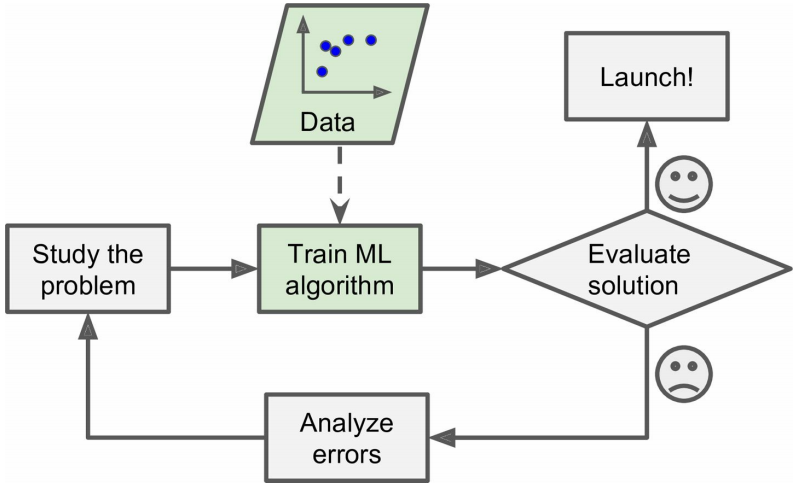
\includegraphics[width=\textwidth]{MLTrainigsphasen}
        \caption{Trainingsprozess (\cite[Figure 1-2]{HandsOnML})}
        \label{fig:MLTrainigsprozess}
    \end{figure}


    \section{Neuronale Netze}
    Neuronale Netze sind eine Form von Machinellem Lernen und die heute am meisten eingesetzte Technik.
    
    \subsection{Aufbau}
    Ein künstliches neuronales Netz ist an das menschliche Gerhin angelehnt und soll dessen neuronales Netz sowie dessen Verhalten abbilden. 
    Dementsprechend besteht ein solches Netz aus mehren Neuronen und Schichten von Neuronen welche über Synapsen miteinander verbunden sind.


    \subsubsection{Neuronen}
    Neuronen bestehen aus Eingängen, auch Dendriten gennant, welche durch eine Eingangsfunktion, eine Aktivierungsfunktionen sowie eine Ausgabefunktion geleitet werden.
    Die Ausgabe eines Neurons besteht daraus dass dieses je nach Eingabe und Art entweder angereg("gefeuert") wird oder nicht.
    
    \begin{figure}[H]
        \centering
        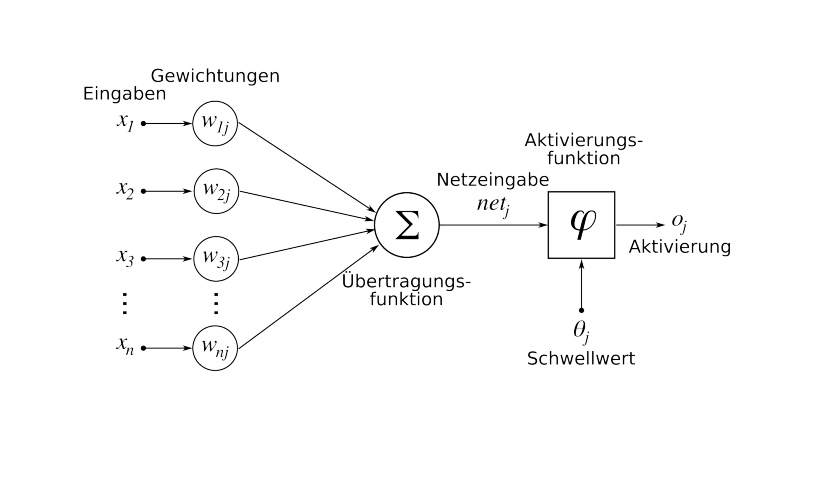
\includegraphics[width=\textwidth]{AufbauNN}
        \caption{Aufbau eines Neurons}
        \label{fig:AufbauNN}
    \end{figure}
    
    \noindent
    Die Eingangsfunktion berechnet aus den verschiedenen Eingängen den effektiven Eingang welcher dann weiter von der Aktivierungsfunktion verarbeitet wird.
    Diese effektive Eingabe ist dann die Netzeingabe in das Neuron.
    Meist wird die Netzaktivität \(net\) einfach als Summe aller Eingänge \(x\) und deren Gewichtungen \(w\) errechnet:
    \begin{equation}
        net = \sum_{i=0}^N x_i w_i
    \end{equation}
    \newline

    \noindent
    Die Aktivierungsfunktion dient zur eigentlichen Auswertung der Eingabe bzw. Netzaktivität.
    Die Aktivierungsfunktionen erzeugt ein Aktiverungspotential welches von der Ausgangsfunktion ausgewertet wird.
    \newline
    
    \noindent
    Die Ausgangsfunktion entscheidet schlussendlich ob das Neuron angeregt wird oder nicht.
    Hierzu wird geprüft ob das Aktivierungspotential der Aktivierungsfunktion einen bestimmten Schwellenwert übersteigt.
    Dieser Schwellenwert wird mithilde einer Schwellenwertfunktion errechnet. 
    Die Schwellenwertfunktion muss monoton wachsend sein, kann jedoch verschiedene Formen annehmen. 
    Sie kann linear Verlaufen wie es beim Perzeptron der Fall ist, nicht-linear oder eine Sprungfunktion sein. 
    Durch eine nciht-lineare Funktion wie die Sigmoid-Funktion lassen sich mächtigere neuronale Netze entwickeln weshalb heuzutage meist eine solche zum Einsatz kommt.


    \subsubsection{Topologie}
    Bei einem neuronalen Netz sind dessen Neuronen über Synapsen, welche bestimmte Kantengewichte bzw. Biases haben, verbunden.
    Durch verschiedene Kantengewichte können Eingänge oder bestimmte Features priorisiert werden. 
    Dies bedeutet, dass Eingänge welche größeren Einfluss auf das erwartetete Ergebnis haben, höher gewichtet werden können und somit stärker in das Ergebnis mit einbezogen werden.
    \newline

    \noindent
    Durch verschiedene Verbindungen zwischen Neuronen ergeben sich verschiedene Topologien von Netzen:
    \begin{description}
        \item[Vorwärts-verkettete Netze], auch feed-forword Netze genannt, bestehen aus verschiedenen Neuronen-Schichten(hidden layers), welche nur mit der nächst höheren Schicht verbunden sind. Somit verlaufen die Daten nur in eine Richtung, vom Eingang zum Ausgang.
        \item[Rekurrente Netze] können auch aus mehreren Neuronen-Schichten bestehen wobei hier auch verbindungen in tiefere Schichten möglich sind. Dies bedeutet, dass auch Ergebnisse von vorherigen Durchläufen des Netztes als Eingang mit einbezogen werden können.
        \item[Voll-vernetzte Netze] sind neuronale Netze, bei denen alle Neuronen mit allen anderen Neuronen vernetzt sind. Wobei hierbei keine wirkliche Struktur erkennbar ist und ein sehr großer Rechenaufwand besteht.
    \end{description}

    \begin{figure}[H]
        \centering
        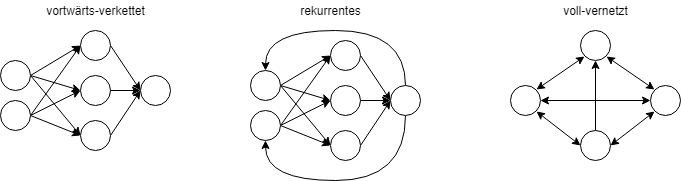
\includegraphics[width=\textwidth]{NetzTopologien}
        \caption{Netztopologien}
        \label{fig:NetzTopologien}
    \end{figure}


    \subsubsection{Lernen}
    Bei neuronalen Netzen ist das vorhandene Wissen durch die Kantengewichte repräsentiert.
    Daraus folgt, dass verschiedene Klassifikationen von neuronalen Netzen, mit derselben Topologie, sich nur von den Kantengewichten abhängt.
    Dementsprechend lernt ein neuronales Netz durch das sequentielle Anpassen der Gewichte.
    Dazu gibt es verschiedene Verfahren wie diese Gewichte angepasst werden können.
    \newline

    \noindent
    Beim \textbf{Backpropagation Lernen} werden in der Trainigsphase die Ergebnissen eines Durchlaufs mit den erwartetten Ergebnissen verglichen und der Ausgabefehler berechnet.
    Mithilfe dieses Fehlers wird nun Schichtweise versucht den Fehler auf einzelene Neuronen bzw. Gewichte bis hin zur Eingabeschicht zurückzuführen.
    Danach werden nun bei verschiedenen Neuronen Änderungen der Gewichte durchgeführt um den Fehler der Ausgabefehlerunktion zu minimieren.
    Hierbei wird für jedes Gewicht eine Änderung berechnet, welche sich aus verschiedenen Parametern, wie die Lernrate zusammensetzt.
    \newline

    \noindent
    Beim \textbf{Batch Lernen} wird anders als beim Backpropagation Lernen nciht nach jeden Durchlauf des Netztes die Gewichte angepasst sondern erst nachdem das Trainingsset komplett durchlaufen wurde.
    Dies führt zu weniger Genauigkeit das nicht auf spezielle Eigenschaften einzelener Einträge eingengangen.
    Jedoch Ist dieses Verfahren sehr viel weniger Rechenaufwand und es können mehr Traningsdaten in gleicher Zeit einbezogen werden.
    
    \subsubsection{Perzeptron}
    Ein sehr einfaches neuronales Netz ist das Perzeptron, welches 1958 von Frank Rosenblatt entwickelt wurde.
    Das Perzeptron besteht aus zwei Eingabeparametern, welche in ein Neuron gegeben werden und von diesem mithilfe der Kantengewichte und der Aktivierungsfunktion eine Ausgabe liefert.

    Ein Beispiel ist die Abbildung des boolschen "`Und"'-Operators welche wie in Abbildung \ref{fig:PerzeptronAND} mit einem Neuron dargestellt werden kann.
    Jedoch können mit einem Neuron nur sehr einfache Funktionen abgebildet werden. 
    Komplexere Funktionen können über mehrere Neuronen bzw. mehrere Schichten von Neuronen abgebildet werden.

    \begin{figure}[H]
        \centering
        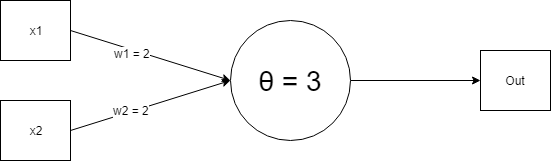
\includegraphics[width=\textwidth]{Perzeptron}
        \caption{UND-Operator als Perzeptron}
        \label{fig:PerzeptronAND}
    \end{figure}

    \begin{table}[H]
        \centering
        \begin{tabular}{|l|l|l|l|}
            \hline
            x1 & x2 & \( (x_1 * w_1) + (x_2 * w_2) \) & out \\
            \hline
            0 & 0 & \( (0 * 2) + (0 * 2) = 0 < 3 \) & 0 \\
            \hline
            0 & 1 & \( (0 * 2) + (1 * 2) = 2 < 3 \) & 0 \\
            \hline
            1 & 0 & \( (1 * 2) + (0 * 2) = 2 < 3 \) & 0 \\
            \hline
            1 & 1 & \( (1 * 2) + (1 * 2) = 4 < 3 \) & 1 \\
            \hline
        \end{tabular}
        \caption{Wahrheitstabelle des Perzeptron}
        \label{tabl:Perzeptron}
    \end{table}

    \subsection{CNN - Convolutional Neural Network}
    \subsection{RNN - Recurrent Neural Network}



\section{Physikalische Grundlagen zur Netzaktivität} \label{physikalischeGrundlagen}

\section{Erhebung der Messdaten} \label{Messdaten}

    Um aussagekräftige Analysen und Klassifikationen über ein Stromnetz bzw. die Geräte in einem Stromnetz mit Maschinellem Lernen machen zu können, werden viele Trainings- und Testdaten benötigt.
    Die Daten bestehen aus verschiedenen physikalische Größen, die zu einem bestimmten Zeitpunkt in einem Stromnetz auftreten.
    Zu diesen Größen gehört die allgemeine Netzspannung, die Netzfrequenz sowie sieben harmonischen Oberwellen (vgl. \ref{physikalischeGrundlagen}).
    Um einen allgemeinen Überblick über den Verlauf der Netzaktivität zu erhalten sowie verschiedene Zeiten und Geräte vergleichen zu können, müssen Daten über lange Zeiträume erhoben werden.\\
    \newline
    Zur Erhebung der Werte zur Netzaktivität wurde ein WeSense-Messgerät\footnote{http://www.wesense-app.com/home-en/} verwendet.
    Dieses Gerät misst alle benötigten Werte und sendet diese über einen MQTT-Broker\footnote{Message Queuing Telemetry Transport} an einen Service von WeSense, welcher dann die Daten aufbereitet und in einer MSSQL Datenbank abspeichert.
    Die Werte werden sekündlich gemessen und in die Datenbank gespeichert, weshalb zunächst in eine row-based Datenbank gespeichert wird und später dann die Daten in eine column-based Datenbank zur schnellen Abfrage überführt werden.
    \newline

    \begin{figure}[h]
        \centering
        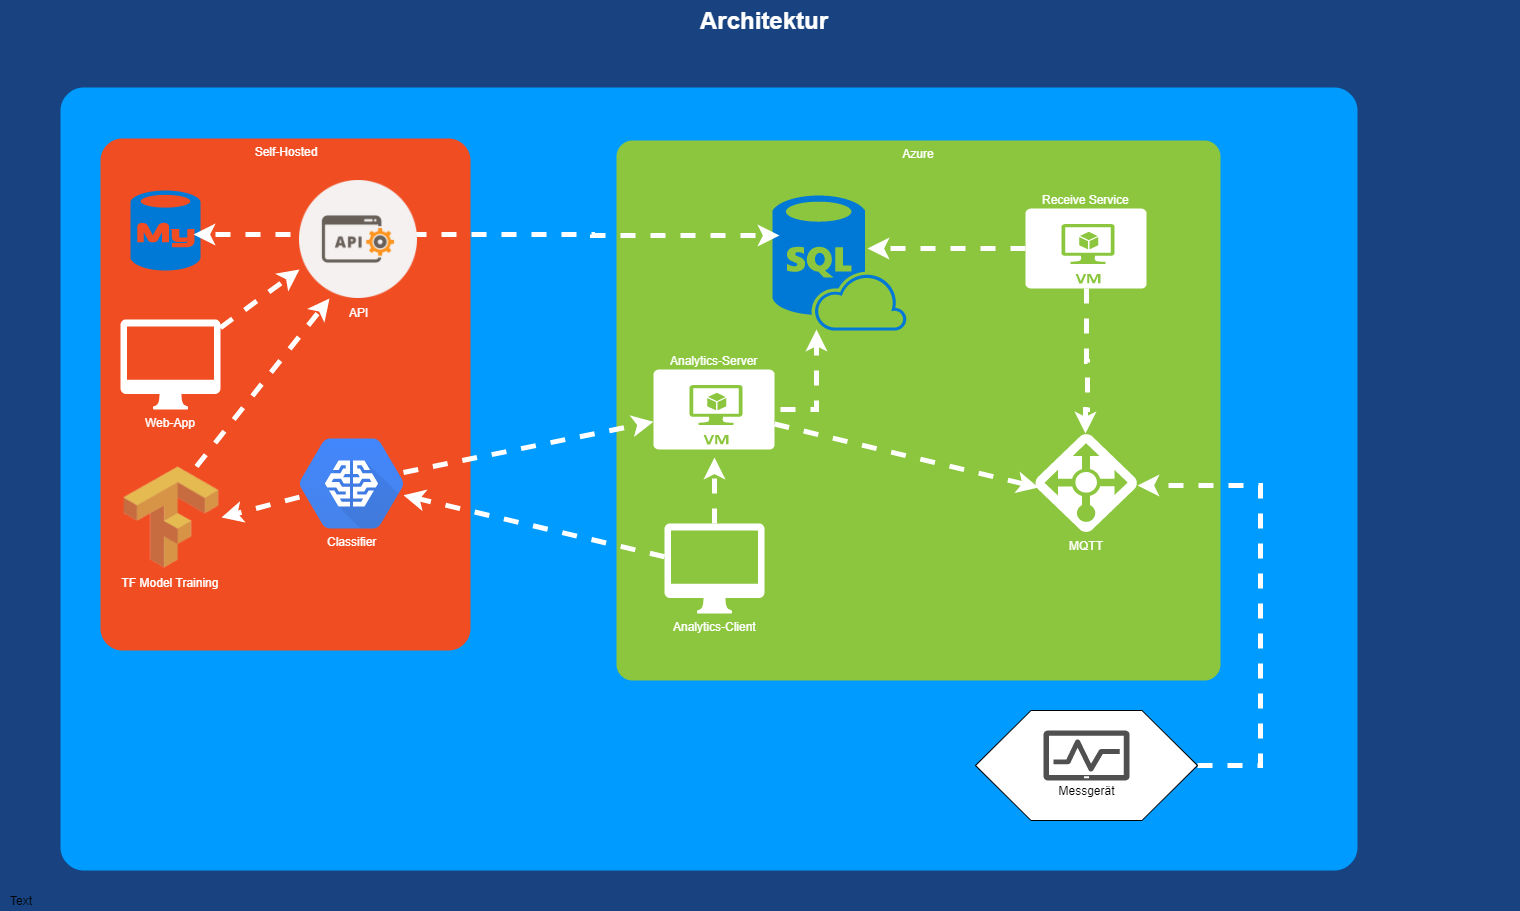
\includegraphics[width=1.0\textwidth]{Architecture}
        \caption{Complete Architecture}
        \label{fig:Architecture}
    \end{figure}

    \subsection{Klassifikation der Messdaten}

        Durch die oben beschriebene Erhebung sind die physikalischen Werte zu bestimmten Zeitpunkten bestimmt worden.
        Zusätzlich wird nun zur Identifikation der Geräte sowie zum Maschinellen Lernen, genau definierte Zeiträume benötigt in denen bestimmte Geräte aktiv waren.
        Dies bedeutet, dass jedem Zeitpunkt ein oder mehrere Geräte zugewiesen werden. \\
        \newline
        Um diese gelabelten Daten zu erheben gibt es verschiedene Möglichkeiten.
        Die Daten können entweder durch eine Person, welche Zeiten zu denen sicher Geräte aktiv waren manuell erfasst, oder durch eine Maschine automatisch erhoben werden.
        Jedoch wird zur automatischen Erhebung ein weiteres Gerät benötigt, welches zwischen dem zu messenden Gerät und dem Stromnetz zwischengeschalten wird und sobald Strom fließt Daten erfasst.
        Somit werden die manuell durch eine Person erfasst.\\
        \newline
        Hierzu wurde eine progressiv Web-App(vgl. Abbildung \ref{fig:WebApp1}) mit einer einfachen MySQL-Datenbank erstellt, mit der die Daten sehr einfach erfasst und abgespeichert werden können.

        \begin{figure}[h]
            \centering
            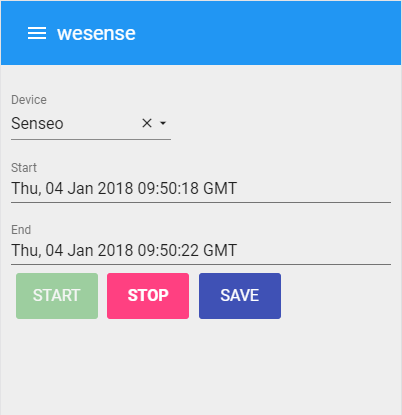
\includegraphics[width=0.5\textwidth]{WesenseConveyWebApp}
            \caption{Screenshot der progressive Web-App}
            \label{fig:WebApp1}
        \end{figure}

\section{Visualisierung}\label{VisualisierungWebApp}

        Zusätzlich zur manuellen Erhebung der Daten wurden zur besseren Analyse der Daten verschiedene Visualisierungsmöglichkeiten implementiert.
        Zum einen können die verschiedenen Physikalischen Größen eines gelabelten Gerätes zu einem bestimmten Zeitpunkt miteinander verglichen werden.
        Außerdem können bestimmte Größen zu verschiedenen gelabelten Zeiträumen eines Gerätes verglichen und analysiert werden.
        Durch diese Visualisierung können sehr gut und genau Gemeinsamkeiten in verschiedenen Größen oder Zeiten erkannt werden.\\
        \newline
        Es werden verschiedene Diagramme sowie Normalisierungen der Daten zur Analyse bereitgestellt.
        Es besteht die Möglichkeit die Daten in einem Liniendiagramm sekündlich oder in frei wählbaren zusammengefassten Datenpunkten, sogennannten Klassen, anzuzeigen.
        Des weiteren können Histogramme mit verschiedenen Klassen gewählt werden.

        \begin{figure}[h]
            \centering
            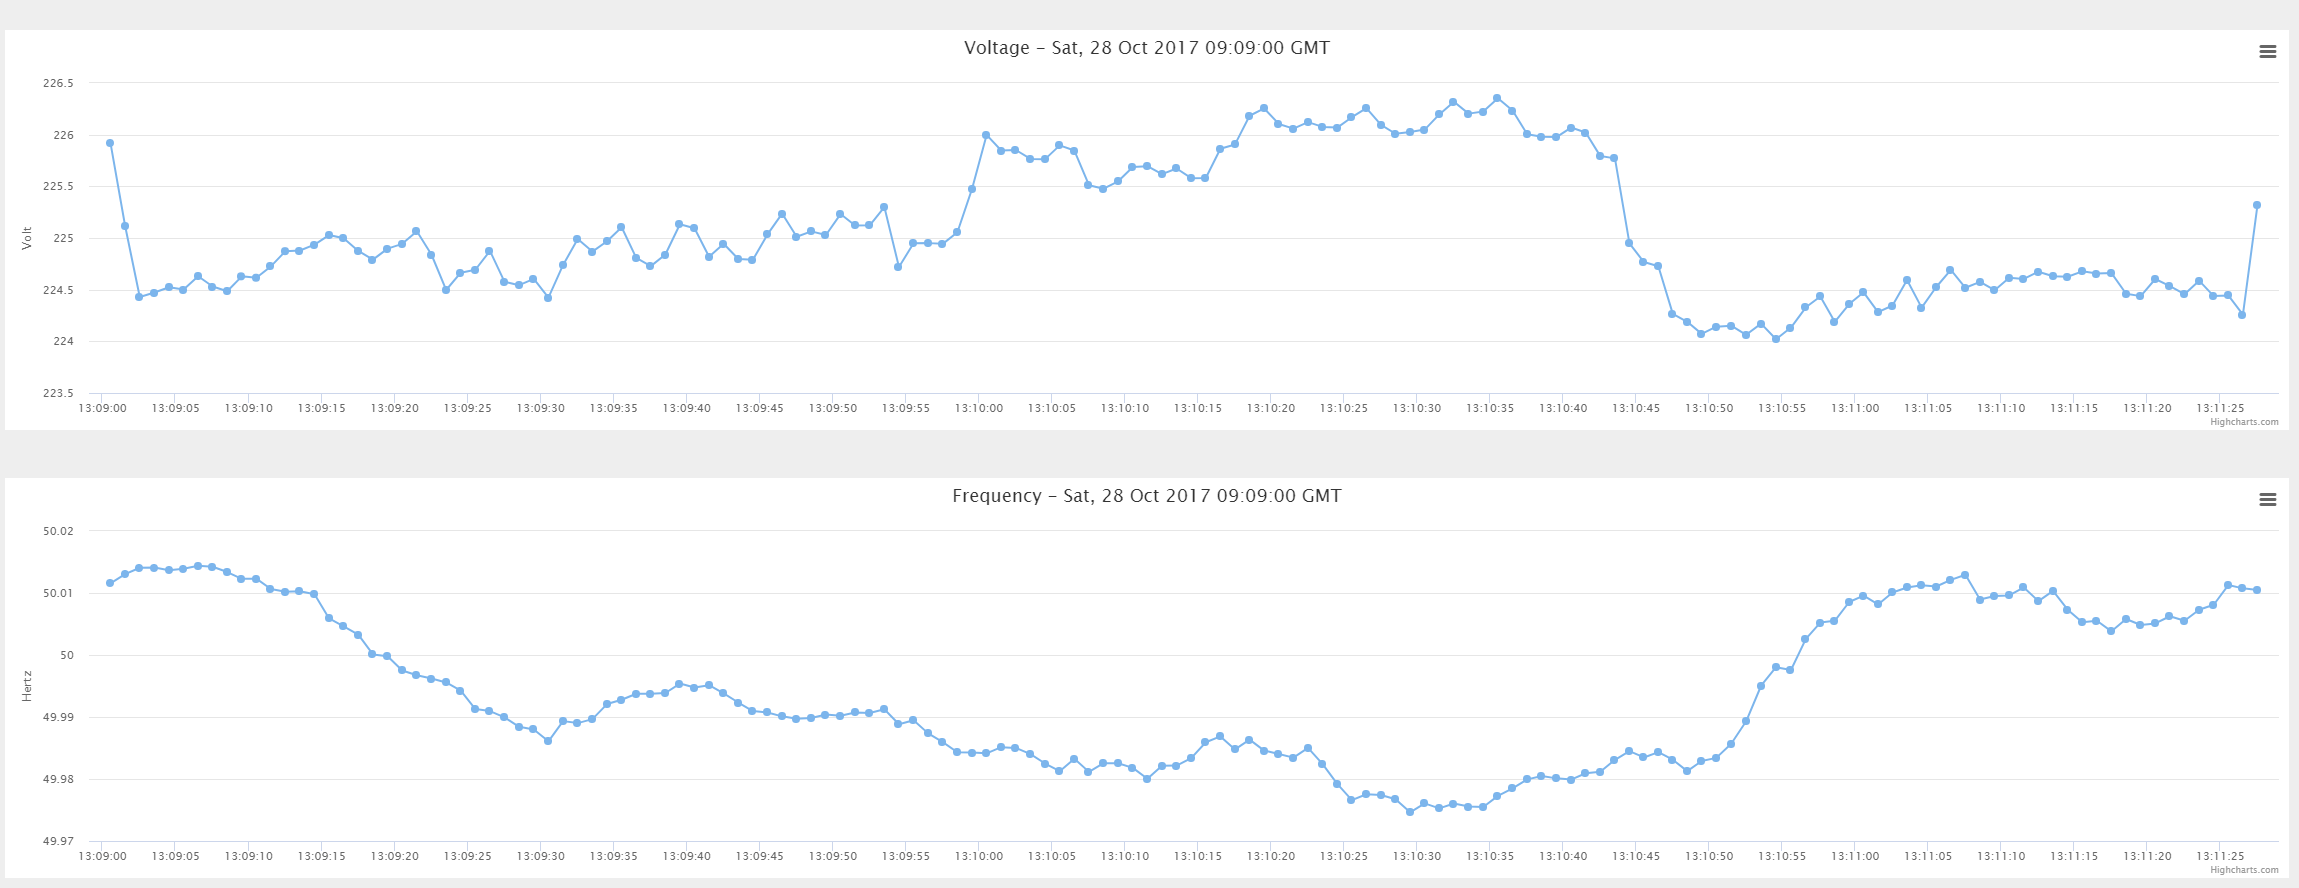
\includegraphics[width=0.75\textwidth]{WesenseConveylineChart}
            \caption{Screenshot eines gelabelten Zeitraumes aus der Web-App}
            \label{fig:WebApp2}
        \end{figure}

\chapter{Ausführung}

    Dieses Kapitel beschreibt die Vorgehensweise von der ersten manuellen Analyse der Daten bis zum fertigen Produkt.
    Als Beispielprodukt für die Klassifizierung wurde eine Senseo Kaffeemaschine gewählt, da durch häufige Benutzung viele Daten erhoben werden können. 
    Außerdem wurde eine Mikrowelle als zweite Gerät mit wenigen Daten gewählt um verschiedene Parameter und Kennzahlen zu vergleichen.
    Hierbei soll die Anzahl der Daten sowie die Klassifikation von mehreren Geräten innerhalb eines Neuronalen Netzes untersucht werden.

\section{Manuelle Analyse} \label{ManuelleAnalyse}

    Zur manuellen Analyse der Daten wird das in \ref{VisualisierungWebApp} beschriebene Tool verwendet.
    Zunächst werden sehr aussagenkräftige Größen wie die Spannung oder die Frequenz der Kaffeemaschine verwendet und mit anderen aktiven Zeiträumen der Kaffeemaschine verglichen.
    Hierbei kann ein sehr spezifischer Verlauf der Spannung erkannt werden.\\ 
    Wie in Schaubild ref{fig:Spannungsverlauf} zu sehen ist, ist die Kurve zu Beginn start fallend und verbleibt dann eine gewissen Zeit auf diesem Tief. 
    nach einem längeren steigenden Abschnitt fällt die Kurve wieder bis der Zubereitungsvorgang beendet wurde und wieder steigt.\\
    \newline
    Diesem Verlauf können nach mehreren Beobachtungen bestimmte Vorgänge einer Kaffeezubereitung zugeordnet werden.
    Zu Beginn der Kaffeezubereitung wird die Kaffeemaschine manuell eingeschaltet. 
    Dies führt automatisch zum erwärmen des Brühwassers, welches dem ersten Fallen der Kurve zugeordnet werden kann. 
    Da dort viel Energie benötigt um das Wasser zu erhitzen steigt der Stromverbrauch der Kaffeemaschine stark an und somit fällt die Netzspannung stark ab.
    Die Netzspannung bleibt solange auf einem gewissen Tiefpunkt mit minmaler Netzschwankung bis das Wasser erwärmt wurde und ein weiterer manueller Schritt zum fortfahren des Prozesses notwendig ist.\\
    Nach Wahl der Tassengröße wird dann der Brühvorgang gestartet. 
    Dabei wird das erhitzte Wasser mit einem gewissen Druck durch einen Kaffeepad gepresst. 
    Da dieser Druck bei der Senseo Kaffeemaschine durch eine elektronische Pumpe erzeugt wird, sinkt demnach die Netzspannung wird ab bis der komplette Kaffee durch gelaufen ist.
    Somit kann die Zweite Tiefpunktphase dem ``Pressvorgang'' der Kaffeemaschine zugeordnet werden.\\
    \newline
    
    \begin{figure}[H]
        \centering
        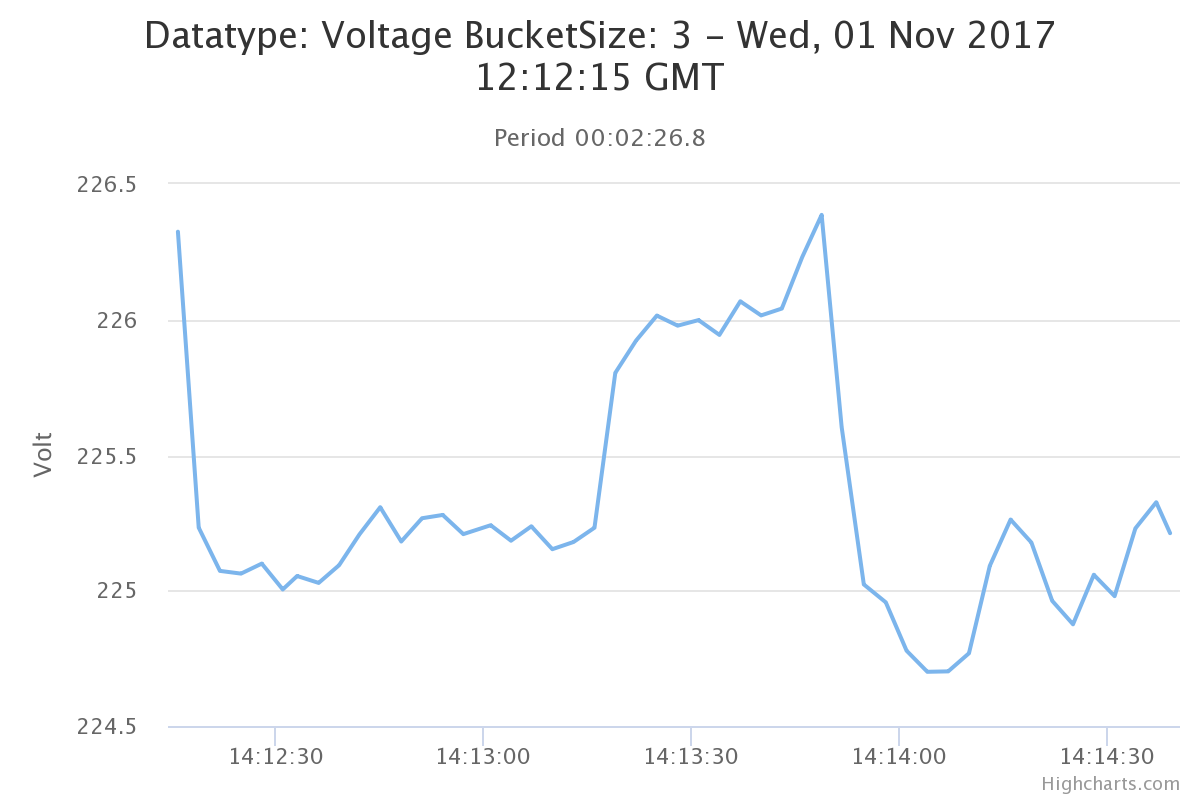
\includegraphics[width=0.8\textwidth]{SpannungsverlaufSenseo1}
        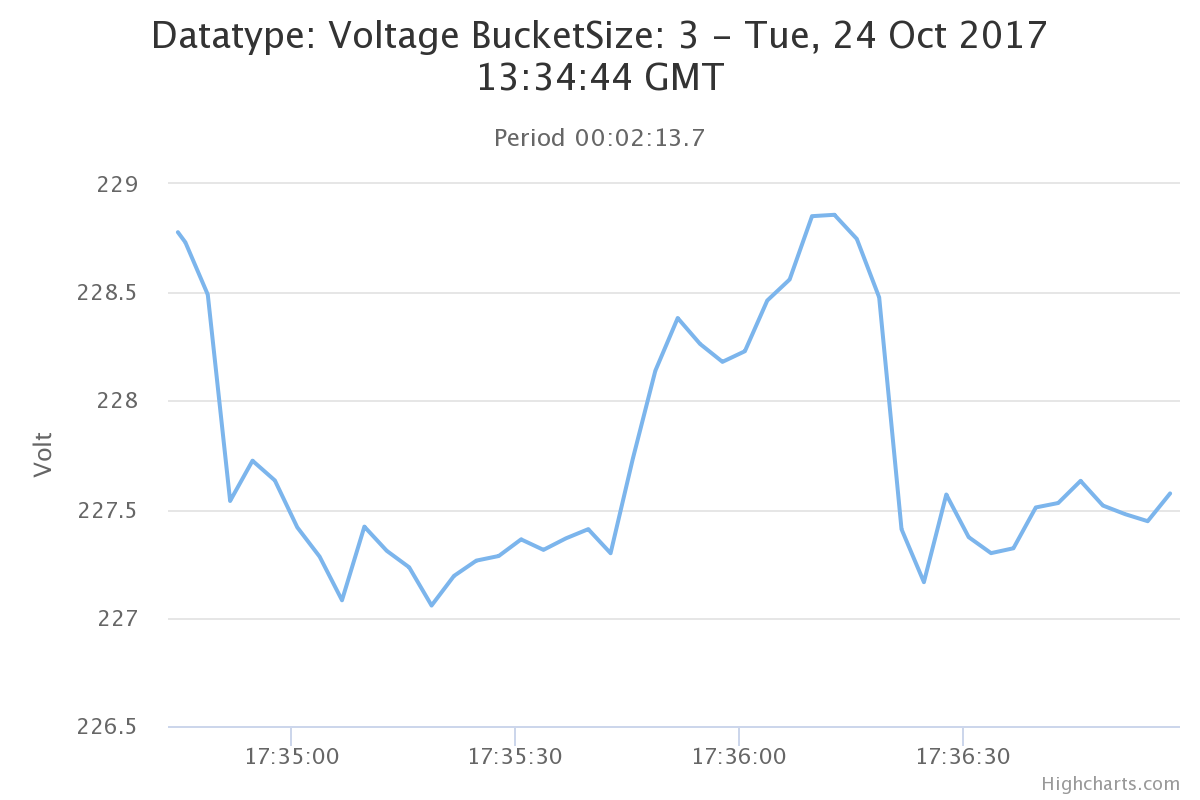
\includegraphics[width=0.8\textwidth]{SpannungsverlaufSenseo2}
        \caption{Spannungsverlauf der Senseo Kaffeemaschine mit einer Klasse von je 3 Datenpunkten zu 2 verschiedenen Zeitpunkten}
        \label{fig:SpannungsverlaufSenseo}
    \end{figure}

    \noindent
    Bei der manuellen Analyse der Mikrowelle können bei Analyse des Spannungs- oder Frequenzverlaufs leider keine hervorstechenden Merkmale oder Gemeinsamkeiten erkannt werden.
    Somit wird die Mikrowelle demnach einen anderen Einfluss auf doe Netzaktivität ausüben.
    Wie bei dem Vergleich der verschiedenen harmonischen Oberwellen zu sehen ist (siehe Schaubild \ref{fig:3OberwelleMikrowelle}), besteht eine große Ähnlichkeit der Kurven der dritten harmonischen Welle.\\
    \newline

    \begin{figure}[H]
        \centering
        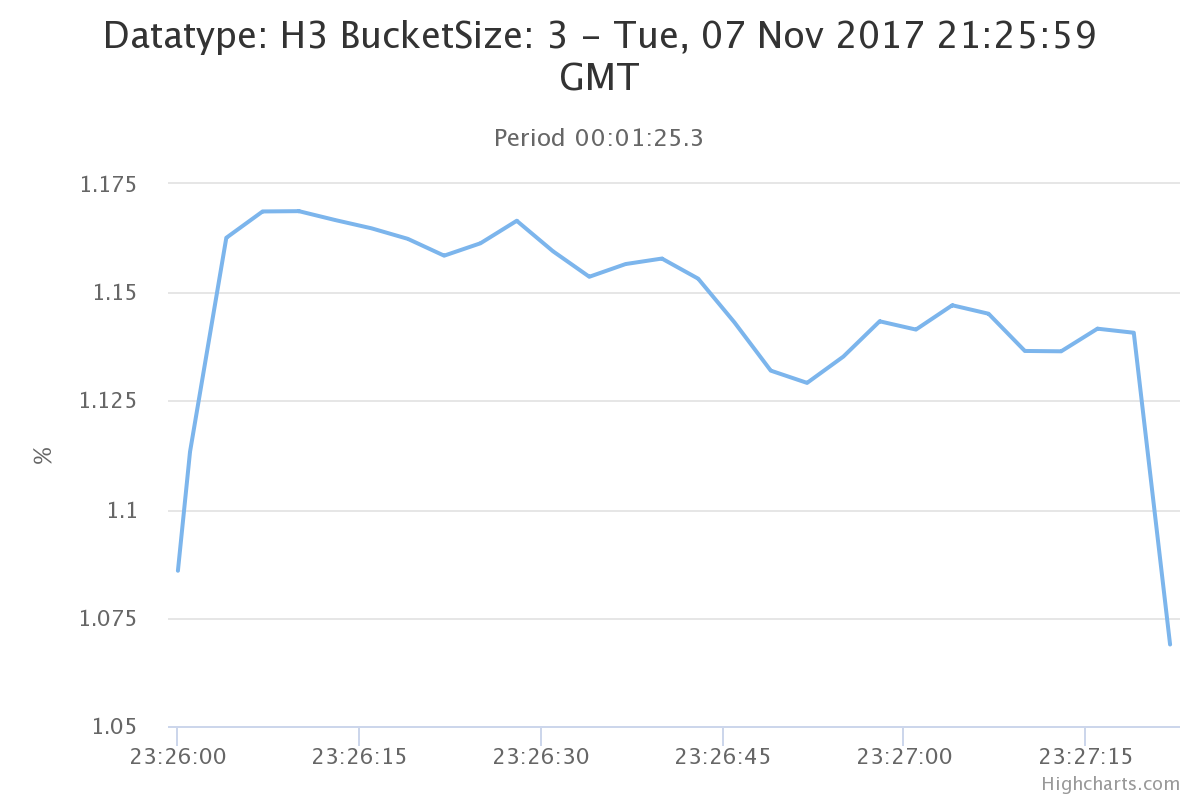
\includegraphics[width=0.8\textwidth]{3OberwelleMikrowelle1}
        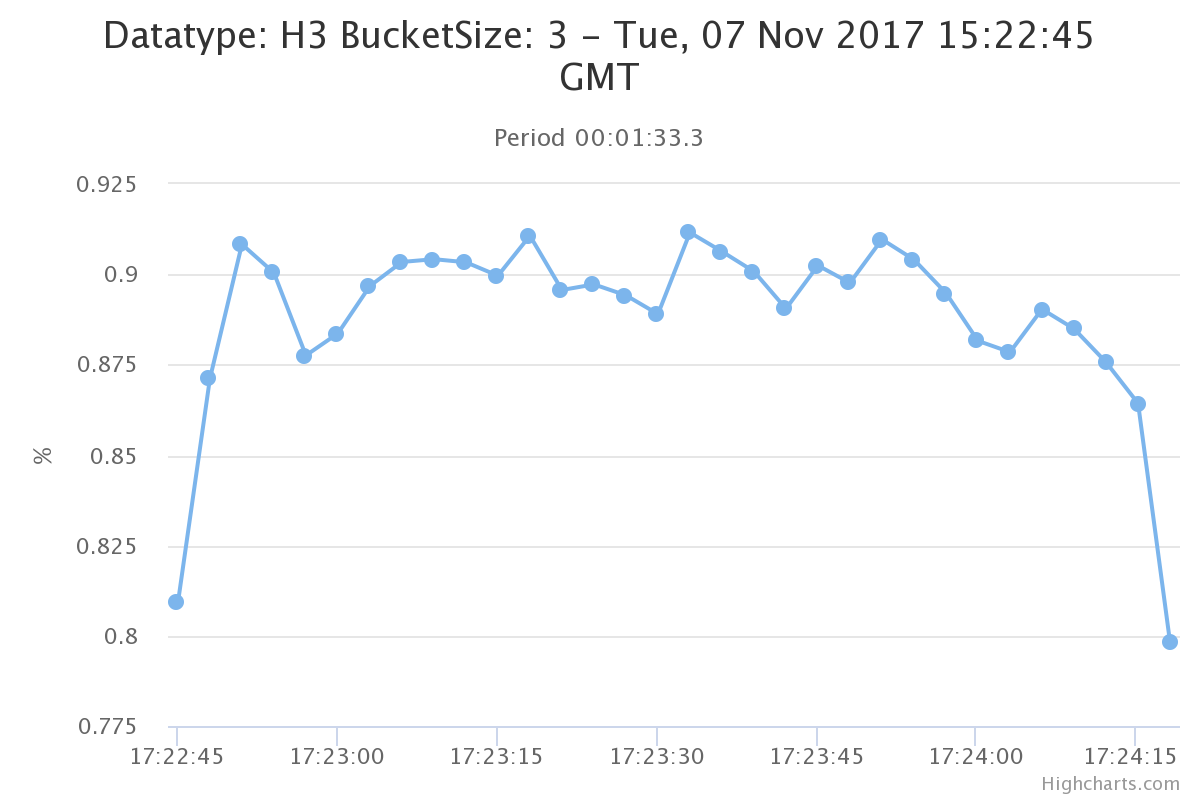
\includegraphics[width=0.8\textwidth]{3OberwelleMikrowelle2}
        \caption{Verlauf der 3. harmonischen Oberwelle einer Mikrowelle mit einer Klasse von je 3 Datenpunkten zu 2 verschiedenen Zeitpunkten}
        \label{fig:3OberwelleMikrowelle}
    \end{figure}

    \noindent
    Wie dieser Abschnitt zeigt können schon mit bloßen Auge bestimmte Auswirkungen der verschiedenen Geräte erkannt werden.
    Auch wenn einige Störungen auftreten und den Verlauf verfälschen, sollte es dennoch möglich sein diese Geräte herauszufiltern.
    Weiterführend wird dieser Prozess automatisiert und verbessert um auch trotz großer Störungen, Geräte präzise klassifizieren zu können. 

\section{Vorbereiten der Daten}\label{VorbereitenDerDaten}
    Um die Klassifizierung der Geräte auf neuronalen Netzen abzubilden müssen die vorhandenen Daten in ein geeignetes Format transformiert werden.
    Dabei gibt es verschiedene Vorraussetzungen zu beachten, sowie verschiedene Möglichkeiten die Daten zu transformieren.\\
    
    \noindent
    Bei konventionellen Neuronalen Netzen werden Eigenschaften Objekten zugewiesen, wobei alle Objekte mit denselben Eigenschaften betitelt werden.
    Ein Beispiel dafür sind Tiere, bei denen anhand von Reproduktion oder Atmung in Säugetiere, Vögel, Reptilien, etc. eingeteilt wird. 
    So können spezielle Tiere wie ein Hund in eine dieser Klassen zugewiesen werden.
    Alle klassifizierten Tiere werden hierbei dieselben Eigenschaftsklassen mit unterschiedlichen Werten zugewiesen.
    Das heißt, dass einem Hund oder einer Taube die Anzahl der Beine und die Reproduktion zugewiesen werden jedoch mit jeweils unterschiedlichen Werten.\\
    
    Durch die in Kapitel \ref{Messdaten} beschriebene Erhebung der Daten, werden die Stromdaten in einem bestimmten Format von der API bereitgestellt.
    Es werden 2 verschiedene Listen zurückgegeben wobei eine die reinen Messdaten enthält und die andere die Labels für diese Daten.\\
    Die reinen Messdaten werden zusammengetragen, indem zu den gelabelten Zeiträumen jeweils alle sekündlich gemessenen Werte des Stromnetzes als eine Matrix eingefügt werden.
    Somit ergibt sich eine drei dimensionale Matrix welche inder ersten Dimension die Zeiträume abbildet, in der zweiten Dimension die sekündliche Zeitreihe und die dritte die vorhandenen physikalischen Größen.

    \begin{lstlisting}[language=Python, caption={Datenstruktur der gelabelten Messdaten, die von der API bereit gestellt wird},label=lst:DatenstrukturGelabelteMessdaten]

[
    [
        [u, f, h3, h5, h7, h9, h11, h13, h15],
        [u, f, h3, h5, h7, h9, h11, h13, h15],
        [u, f, h3, h5, h7, h9, h11, h13, h15],
        ...
    ]
]
    \end{lstlisting}

    Da Neuronale Netze feste Eingabegrößen benötigen, werden die Daten in Batches aufgeteilt.
    Batches bedeutet, dass die Zeitreihe in gleich große Abschnitte aufgeteilt wird.
    Dementsprechend wird die Matrix \( A[m, n, 9] \), zu einer Matrix mit einheitlicher Größe transfomiert, sodass die enstehende Matrix zum Beispiel die Form \( B[m, 20, 9] \) annimt.
    \newline

    \noindent
    Um diese neue Matrix zu erhalten wird folgender Algorithmus auf die alte Matrix angewandt:

    \begin{algorithm}
        \caption{Batch Generierung}
        \begin{algorithmic}[1]
        \Function{GeneriereBatches}{$A,b$}\Comment{A - Matrix, b - Batchgröße}
            \State ${B} = []$
            \For{$i = 0$ to $length(A)$}
                \For{$j = 0$ to $length(A[i]) - b$}
                    \State $start = j$
                    \State $end = j + b$ 
                    \State $I_b = length(B) + 1$
                    \State $B[I_b] = A[i][start : end]$
                \EndFor
            \EndFor
            \State return $B$
        \EndFunction
        \end{algorithmic}
    \end{algorithm}

\section{Neuronales Netz}
    Wie Abschnitt \ref{ManuelleAnalyse} zeigt ist es möglich mit herkömmlichen manuellen Methoden verschiedene Geräte innerhalb eines Verlaufs zu klassifzieren.
    Somit sollte dies auch mit maschinellem Lernen möglich sein.
    \newline

    \noindent
    Um nun die Geräte maschinell zu klassifiziren, werden drei verschiedene "`neuronale Netz"' Modelle erstellt und miteinander verglichen.
    Die drei Modelle beinhalten ein "`Recurrent Neural Network(RNN) "', ein "`Convolutional Neural Network(CNN)"' sowie eine Mischung aus diesen Ansätzen. 
    Bei allen Modellen wurde als Gradientenverfahren die Adam-Optimierung gewählt, da diese bei mehr Rechenaufwand bessere Ergebnisse erzielt.
    \newline

    \noindent
    

    \subsubsection{CNN}
    Grundlegend besteht das \ac{CNN} aus einem "`Input Layer"', drei "`Convolutional Layers"', einem "`Dropout Layer"' sowie einem "`Output Layer"'.
    \newline

    \noindent
    Das "`Input Layer"' ist der Eingang zum neuronalen Netz, welcher die Rohdaten annimmt und an das eigentliche Netz weiterleitet. 
    Es ist ein weiteres "`Convolutional Layer"' und nimmt einen Eingabe-Tensor (Matrix innerhalb eines neuronalen Netzes), welcher an die Batchgröße angepasst ist.
    Dementsprechend hat der Eingabetensor die Form \( A[m, b, 9] \), mit m: Trainingsdatengröße und b: Batchgröße.
    \newline

    \noindent
    Die Eingabe wird dann weitergeleitet an die drei "`Convolutional Layers"', welche mit unterschiedlicher "`Hidden Layer"'-Größe initialisiert werden.
    Wobei die "`Hidden Layer"' größer werden je näher sie topologisch an dem "`Output Layer"' liegen.
    \newline

    \noindent
    Das "`Dropout Layer"' wird eingefügt um die Tensordimension zu verkleinern und somit das Ergebnis zu generalisieren und Overfitting zu vermeiden.
    \newline

    \noindent
    Das "`Output Layer"' wandelt nun die Erkenntnisse der vorherigen Schichten in ein lesbares Fomat um. 
    Hierzu wird ein "`Dense Layer"', welcher ein eindimensionaler Tensor mit einem Feld pro klassifizierbaren Objekt ist. 
    Dies bedeutet, dass dieser Tensor bei einem Klassifizierung von zwei Geräten ein Array mit der Größe 2 ist.     
    
    \begin{figure}[H]
        \centering
        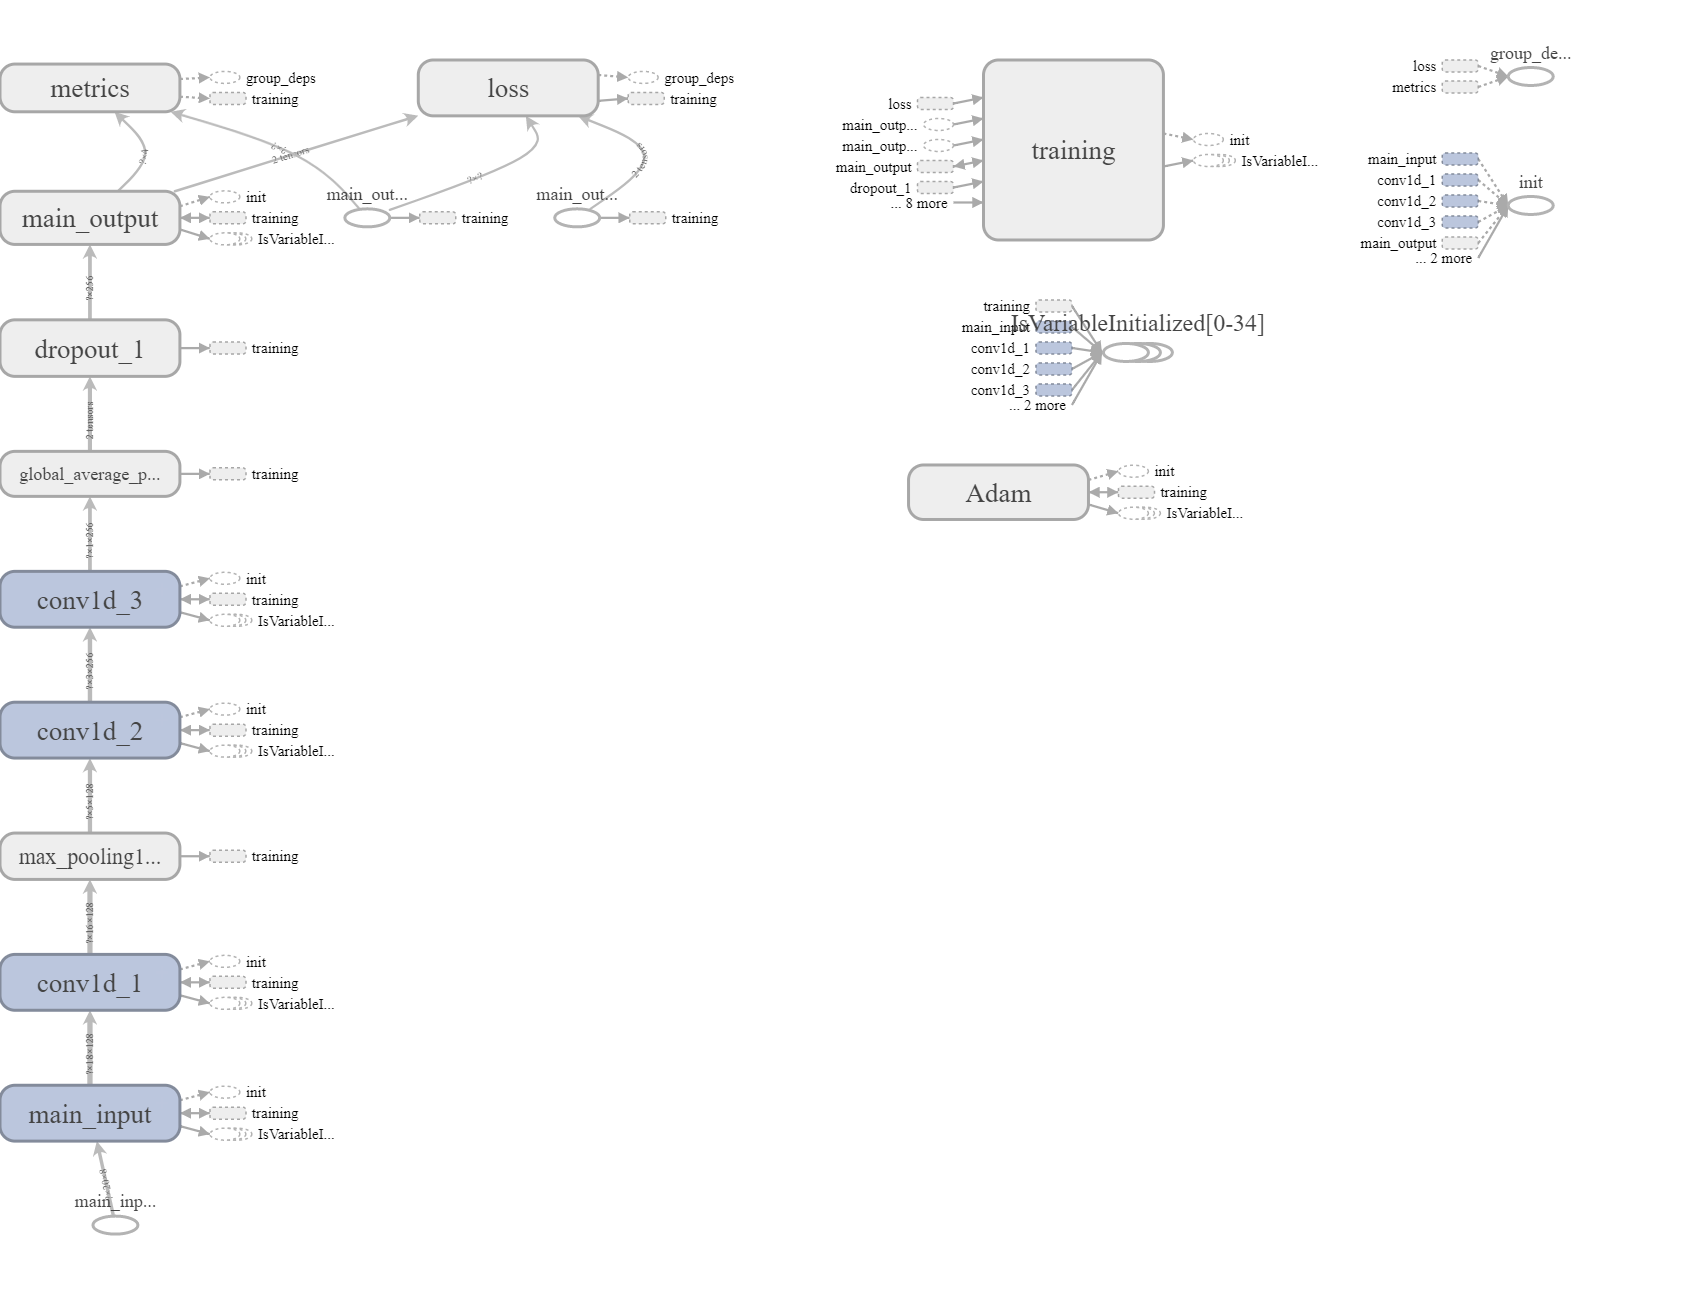
\includegraphics[width=\textwidth]{CNN_Model}
        \caption{Convolutional Neural Network}
        \label{fig:CNN_MODEL}
    \end{figure}

    \subsubsection{RNN}
    Das "`Recurrent Neural Network(RNN) "'- Model besteht aus einem "`Input Layer"', zwei darauffolgende "`LSTM(Long short-term memory) Layer"' und einem "`Ouput Layer"'.\\
    \noindent
    Das "`Input Layer"' ist ein weitereres "`LSTM Layer"' welche denselben Eingabetensor annimt, wie das CNN-Model.\\
    \noindent
    Es folgen zwei weitere "`LSTM Layer"' mit derselben "`Hidden Layer"'-Größe, wie des Eingabe-"`LSTM Layers"'.

    \begin{figure}[H]
        \centering
        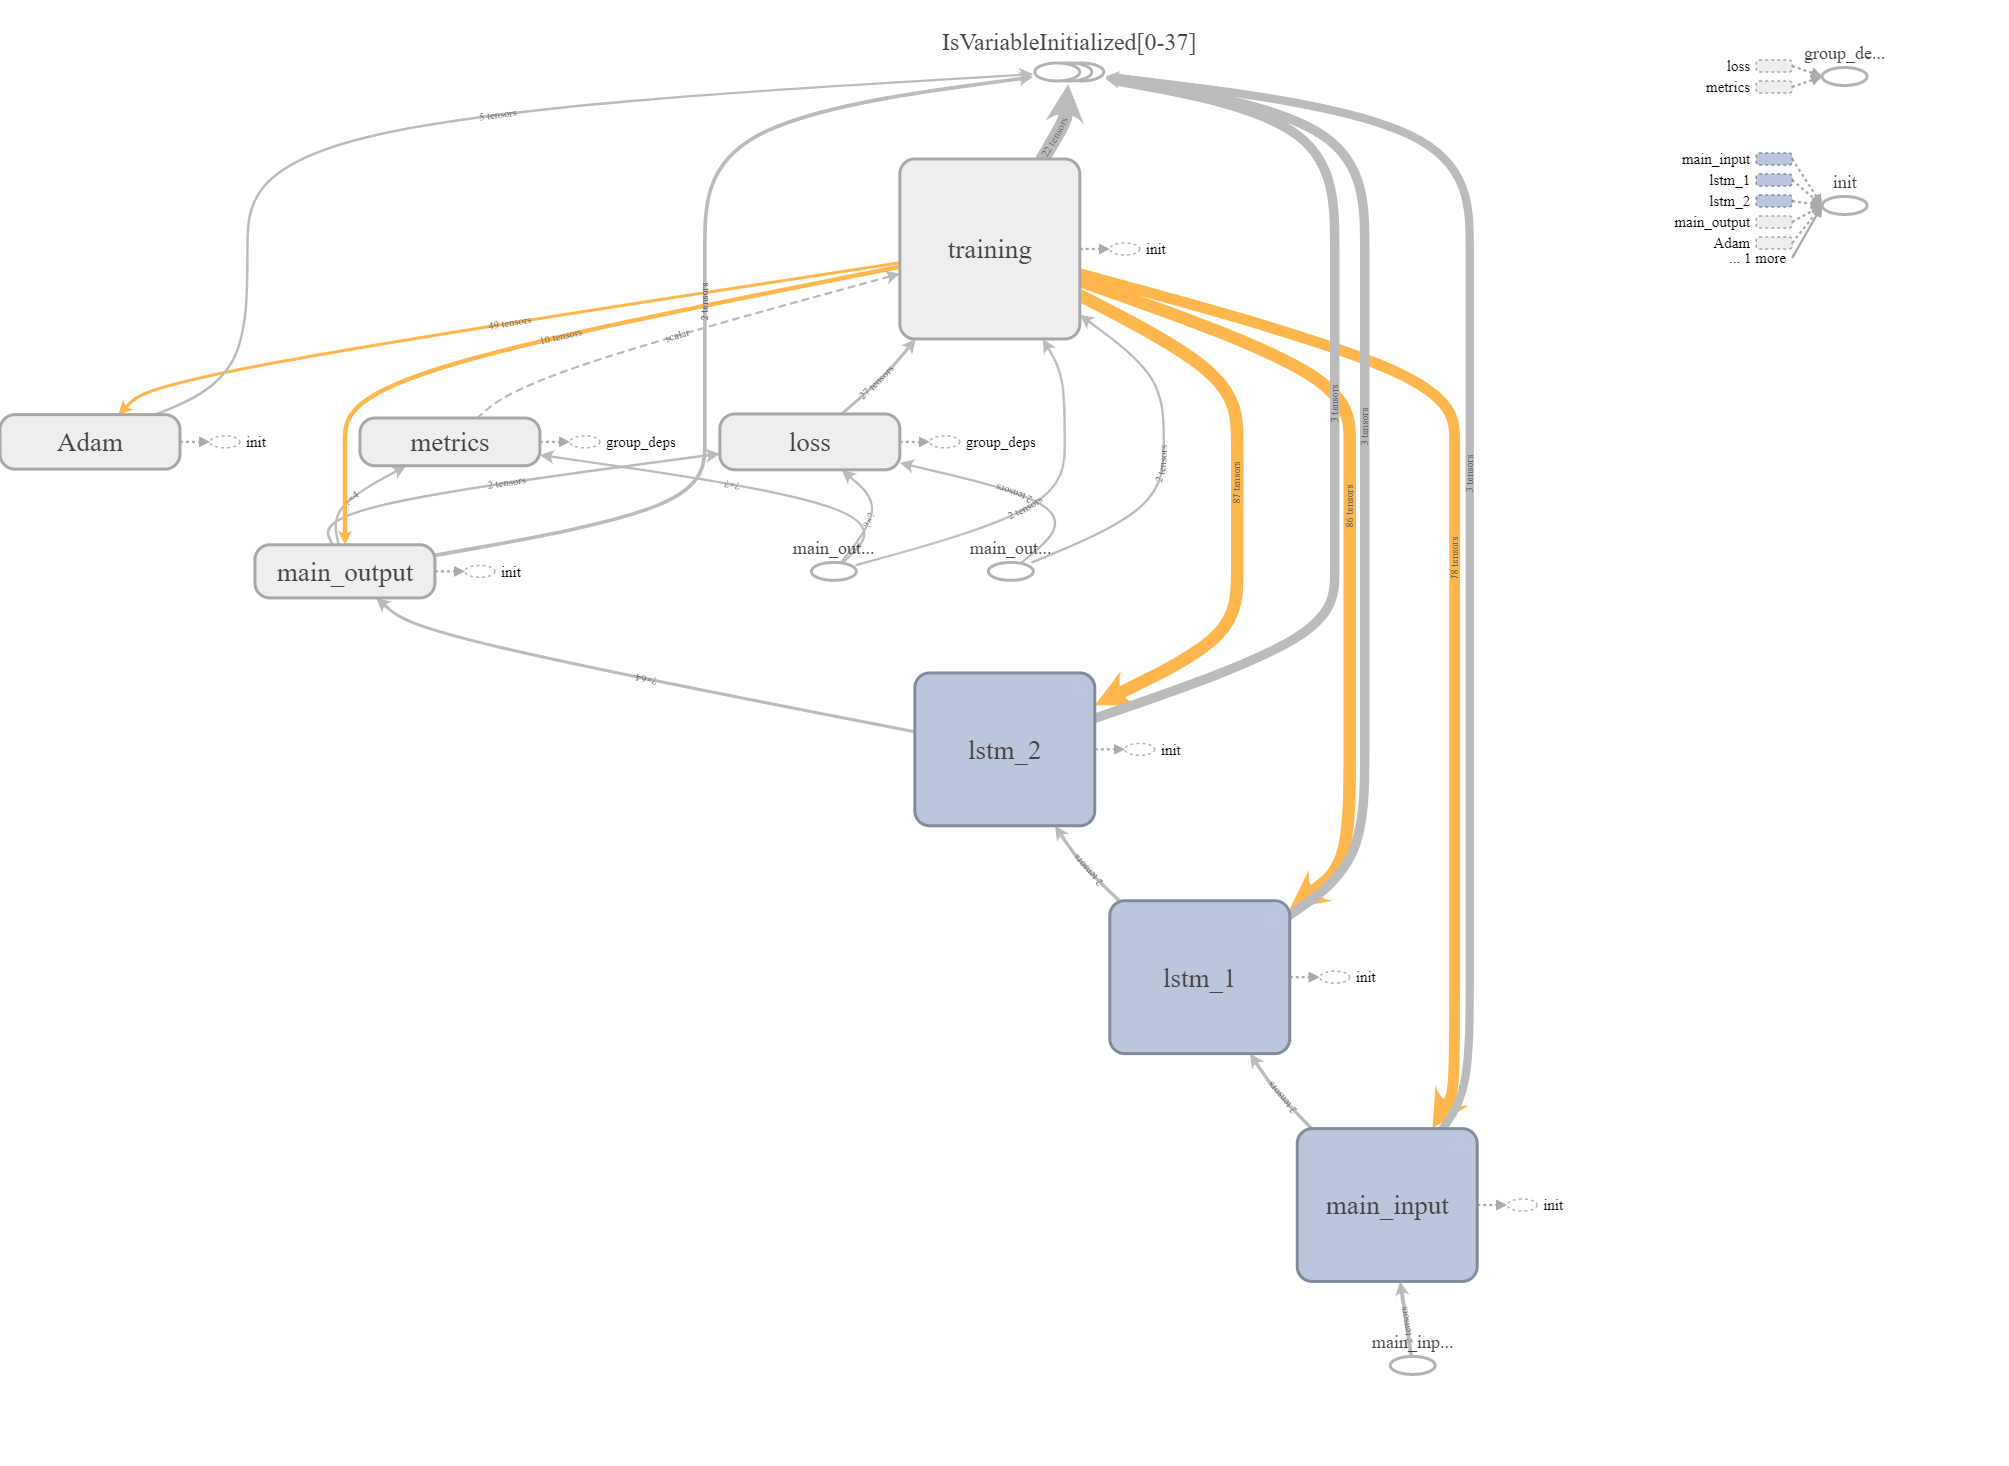
\includegraphics[width=\textwidth]{RNN_Model}
        \caption{Recurrent Neural Network}
        \label{fig:RNN_MODEL}
    \end{figure}

    \begin{figure}[H]
        \centering
        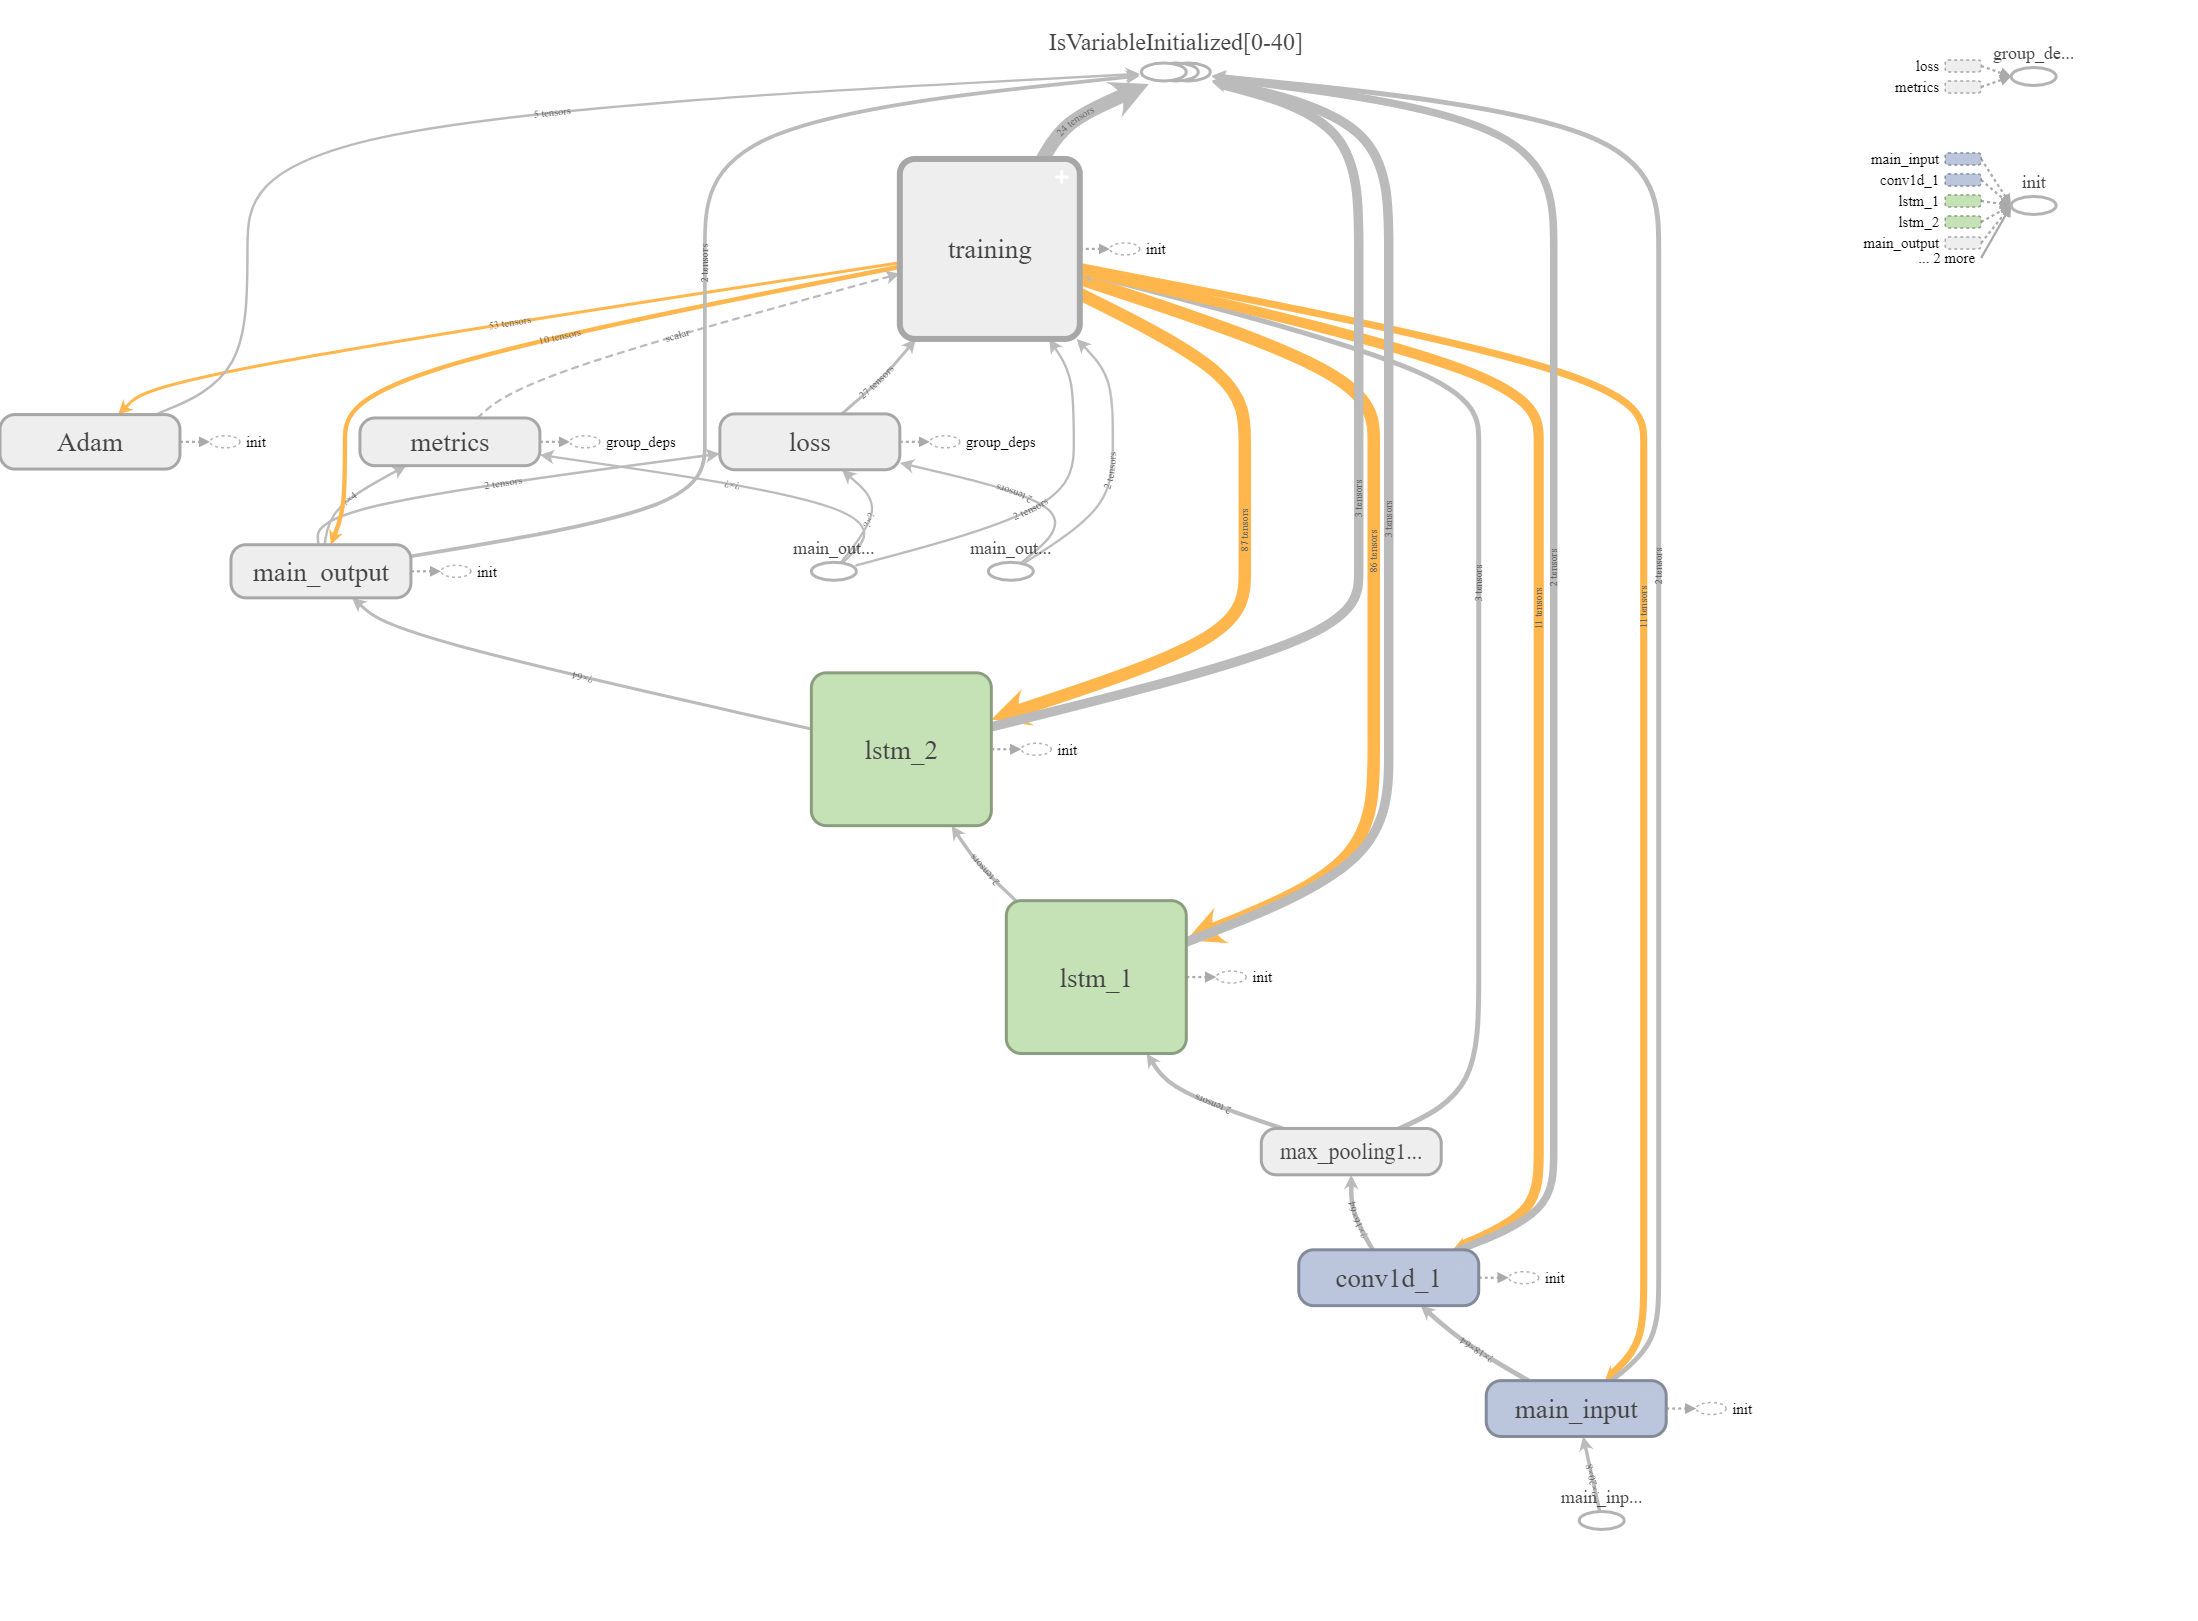
\includegraphics[width=\textwidth]{MIX_Model}
        \caption{Convolutional Neural Network with Recurrent Neural Network}
        \label{fig:MIX_MODEL}
    \end{figure}



    
    % batches von 20 / 30 / 60
    % überlappende batches
    % 1 batch von 20 Datenpunkten pro sekunde --> mehr daten und höhere genauigkeit beim späteren klassifizieren
    % Untransformierte Daten
    % Ableitungen da Verlauf bzw. Kurve entscheidend und nicht rein Werte wie bei Bildern
    % Normalisieren auf Werte zwischen 0 und 1 um Matrizen besser auswerten zu können


\section{Trainingsprozess}

\section{Auswertung der Ergebnisse}
    % verschiedene Batch größen vergleichen
    % verschiedene neuronale Netze vergleichen CNN, RNN, CNN + RNN
    % vllt. verschiedene Aktivierungsfunktionnen Sigmoid / Cross-Entropie / Binary Cross-Entropie

\chapter{Ergebnis}\label{Ergebnis}

    Wie die nachfolgendenen Ergebnisse des Trainingsprozesses zeigen, unterscheiden sich die Ergebnisse der verschiedenen Netze stark.

    Generell zeigen die Ergebnisse, dass ein \ac{CNN} bessere beziehungsweise genauere Ergebnisse ohne Overfitting erzielt als ein \ac{RNN} bei gleichen Parametern.
    Dies führt auch dazu, dass das "`Mixed-Modell"' Ergebnisse zwischen den beiden reinen Modellen liefert.
    Auch sieht man sehr gut, dass ein Model mit einem \ac{RNN} schneller trainiert, jedoch auch sehr früh Overfittet (vgl. Tabelle \ref{tabl:ErgebnisEpoch} ).
    
    \paragraph{Batch} 
    Bei der Wahl der Batchgröße müssen zwei Faktoren für die Bewertung beachtet werden. 
    Wie bei den anderen Parametern sind die Genauigkeiten ein wichtiger Faktor. 
    Hierbei ist zu sehen, dass mit steigender Batchgröße die Genauigkeit prinzipiell steigt, jedoch ein Overfitting bei zu großen Werten eintritt.
    Dies ist auf die Laufzeit der einzelnen Geräte zurückzuführen.
    Der zweite Bewertungsfaktor der Batchgröße ist die Laufzeit(Runtime) der zu klassifizierenden Geräte. 
    Die Batchgröße darf nicht größer sein als die kürzeste Laufzeit eines zu klassifizierenden Gerätes, da sonst zu der Ungenauigkeit des neuronalen Netzes die Ungenauigkeit der Batchgröße hinzukommt. %$$ f = \frac{Batchgröße}{Laufzeit} $$
    Somit sollte trotz besserer Ergebnisse mit großen Batches eine eher kleine Batchgröße gewählt werden.

    \paragraph{Epoche} 
    Mit höherer Epochenanzahl, also mehreren Trainingsdurchläufen mit allen Trainingsdaten sowie Backpropagation lernen, werden alle Modelle besser trainiert und erzielen bessere Ergebnisse.
    Jedoch tritt bei Modellen mit einem \ac{RNN} bei zu großen Trainingsdurchläufen, wie oben beschreiben, Overfitting auf.
    Dies bedeutet, dass bei \ac{RNN}-Modellen weniger Epochen durchlaufen werden sollten als bei \ac{CNN}-Modellen.

    \paragraph{Lernrate}
    Die Lernrate hat bei 20 Epochen nur wenig Einfluss auf das Ergebnis der neuronalen Netze.
    Jedoch besteht bei hoher Lernrate die Gefahr, das Overfitting schneller auftritt oder bestimmte Features durch Zufall zu stark in das Ergebnis einfließen.
    Hier sollte eine kleine Lernrate mit höherer Epochenzahl für besserer Ergebnisse gewählt werden.
    \newline

    \noindent
    Zusammenfassend kann somit festgestellt werden, dass die besten Ergebnisse erzielt werden können, wenn die Lernrate niedrig ist, viele Epochen trainiert wird und eine kleinere Batchgröße gewählt wird.
    Zur Erkennung von Mustern innerhalb einer Zeitserie mit mehreren Features eignet sich im Fall dieser Arbeit ein \ac{CNN} am besten.

    \subsubsection{Batchgröße}

        Lernrate = 0.001\\
        \noindent
        Datentypen = ['u', 'h3', 'h5', 'h7', 'h9', 'h11', 'h13', 'h15']\\
        \noindent
        Epochen = 30\\

        \begin{table}[H]
            \centering
            \begin{tabular}{|c|c|c|c|}
                \hline
                Model & Batchgröße & Genauigkeit & Validierungsgenauigkeit \\
                \hline
                CNN & 20 & 96,62\% & 95,16\% \\
                \hline
                RNN & 20 & 84,68\% & 84,70\% \\ 
                \hline
                MIX & 20 & 89,53\% & 89,24\% \\ 
                \hline
                \hline
                CNN & 30 & 97,97\% & 95,05\% \\ 
                \hline
                RNN & 30 & 89,31\% & 89,02\% \\ 
                \hline
                MIX & 30 & 94,28\% & 92,96\% \\ 
                \hline
                \hline
                CNN & 40 & 98,85\% & 98,94\% \\ 
                \hline
                RNN & 40 & 92,85\% & 92,05\% \\
                \hline
                MIX & 40 & 96,90\% & 96,92\% \\ 
                \hline
                \hline
                CNN & 50 & 99,21\% & 96,95\% \\ 
                \hline
                RNN & 50 & 95,82\% & 96,21\% \\ 
                \hline
                MIX & 50 & 98,74\% & 98,79\% \\ 
                \hline
                \hline
                CNN & 60 & 99,49\% & 91,63\% \\ 
                \hline
                RNN & 60 & 96,61\% & 96,39\% \\ 
                \hline
                MIX & 60 & 99,17\% & 98,99\% \\
                \hline
            \end{tabular}
            \caption{Ergebnis: Batchgröße}
            \label{tabl:ErgebnisBatchsize}
        \end{table}

    \subsubsection{Epochen}

        Lernrate = 0.001\\
        \noindent
        Datentypen = ['u', 'h3', 'h5', 'h7', 'h9', 'h11', 'h13', 'h15']\\
        \noindent
        Batchgröße = 20\\

        \begin{table}[H]
            \centering
            \begin{tabular}{|c|c|c|c|}
                \hline
                Model & Epochen & Genauigkeit & Validierungsgenauigkeit \\
                \hline
                CNN & 10 &  87,38\% & 87,36\%  \\ 
                \hline
                RNN & 10 &  82,01\% & 81,22\%  \\ 
                \hline
                MIX & 10 &  83,28\% & 82,76\% \\ 
                \hline
                \hline
                CNN & 20 &  93,93\% & 92,09\%  \\ 
                \hline
                RNN & 20 &  84,41\% & 84,00\% \\ 
                \hline
                MIX & 20 &  86,68\% & 86,15\%  \\ 
                \hline
                \hline
                CNN & 30 &  96,75\% & 95,72\%  \\ 
                \hline
                RNN & 30 &  84,88\% & 84,57\%  \\ 
                \hline
                MIX & 30 &  88,23\% & 87,87\%  \\ 
                \hline
                \hline
                CNN & 40 &  98,18\% & 96,76\% \\ 
                \hline
                RNN & 40 &  85,18\% & 84,46\%  \\ 
                \hline
                MIX & 40 &  90,90\% & 89,72\%  \\ 
                \hline
                \hline
                CNN & 50 &  98,86\% & 97,50\%  \\ 
                \hline
                RNN & 50 &  85,80\% & 84,80\%  \\ 
                \hline
                MIX & 50 &  91,93\% & 91,10\%  \\ 
                \hline
                \hline
                CNN & 60 &  99,15\% & 98,58\%  \\ 
                \hline
                RNN & 60 &  85,67\% & 85,66\%  \\ 
                \hline
                MIX & 60 &  94,09\% & 90,53\%  \\ 
                \hline
                \hline
                CNN & 70 &  99,39\% & 99,02\%  \\ 
                \hline
                RNN & 70 &  86,63\% & 86,09\%  \\ 
                \hline
                MIX & 70 &  94,52\% & 92,94\%  \\ 
                \hline
                \hline
                CNN & 80 &  99,57\% & 99,27\%  \\ 
                \hline
                RNN & 80 &  86,22\% & 86,81\%  \\ 
                \hline
                MIX & 80 &  95,56\% & 93,98\%  \\ 
                \hline
                \hline
                CNN & 90 &  99,89\% & 99,63\%  \\ 
                \hline
                RNN & 90 &  87,64\% & 86,67\%  \\ 
                \hline
                MIX & 90 &  95,96\% & 94,42\%  \\ 
                \hline
                \hline
                CNN & 100 & 99,49\% & 99,37\%  \\ 
                \hline
                RNN & 100 & 87,29\% & 86,43\%  \\ 
                \hline
                MIX & 100 & 97,39\% & 96,46\% \\
                \hline

            \end{tabular}
            \caption{Ergebnis: Epochen}
            \label{tabl:ErgebnisEpoch}
        \end{table}

    \subsubsection{Lernrate}

        Datentypen = ['u', 'h3', 'h5', 'h7', 'h9', 'h11', 'h13', 'h15']\\
        \noindent
        Batchgröße = 20\\
        \noindent
        Epochen = 30\\

        \begin{table}[H]
            \centering
            \begin{tabular}{|c|c|c|c|}
                \hline
                Model & Lernrate & Genauigkeit & Validierungsgenauigkeit \\
                \hline
                CNN & 0.0001 & 97,13\% & 95,55\% \\
                \hline
                RNN & 0.0001 & 84,54\% & 84,91\% \\
                \hline
                MIX & 0.0001 & 88,45\% & 88,43\% \\
                \hline
                \hline
                CNN & 0.001  & 96,65\% & 93,85\% \\
                \hline
                RNN & 0.001  & 84,98\% & 84,34\% \\
                \hline
                MIX & 0.001  & 90,17\% & 89,02\% \\
                \hline
                \hline
                CNN & 0.01   & 96,91\% & 93,42\% \\
                \hline
                RNN & 0.01   & 84,67\% & 84,84\% \\
                \hline
                MIX & 0.01   & 89,71\% & 89,41\% \\
                \hline
                \hline
                CNN & 0.1    & 96,51\% & 95,50\% \\
                \hline
                RNN & 0.1    & 85,06\% & 84,62\% \\
                \hline
                MIX & 0.1    & 89,46\% & 88,51\% \\
                \hline
            \end{tabular}
            \caption{Ergebnis: Lernrate}
            \label{tabl:ErgebnisLernrate}
        \end{table}   


    \subsection{Auswertung der Ergebnisse}

        Nach Anwendung des in \ref{Auswertungsalgorithmus} beschriebenen Algorithmus ergeben sich die nachfolgenden Abbildungen der verschiedenen neuronalen Netze.
        Die Abbildungen zeigen die jeweiligen klassifizierten Geräte jeden Zeitpunktes von Abbildung \ref{fig:ResultClassificationPeriod}.
        Hierbei zeigt die x-Achse den Zeitpunkt und die y-Achse das Gerät, wobei 
        y: 0 \( \Rightarrow \)  "`Senseo Kaffeemaschine"',\\
        \noindent
        y: 1 \( \Rightarrow \)  "`Mikrowelle"',\\
        \noindent
        y: 2 \( \Rightarrow \)  "`Bosch Vollautomat"',\\
        \noindent
        und y: 3 \( \Rightarrow \) "`Kein aktives bekanntes Gerät"'.
        \\
        
        \noindent
        Die Abbildungen zeigen unterschiedliche Bewertungen beziehungsweise Klassifizierungen der Zeitpunkte.
        Gut können die Gemeinsamkeiten aller drei Klassifizierungen erkannt werden.
        Trotz der Einbeziehung vieler verschiedener Ergebnisse (vgl Algorithmus \ref{Auswertungsalgorithmus}), gibt es noch viele kleine Ausreißer.
        Diese Ausreißer sind bei allen Modellen unterschiedlich verteilt und auch mit unterschiedlicher Länge.
        Jedoch kann man sehr gut sehen, dass alle drei einen großen gemeinsamen Abschnitt haben (ca. y = [30, 190]), wo die "`Senseo Kaffeemaschine"' erkannt wurde.
        Somit kann mit hoher Wahrscheinlich davon ausgegangen werden, dass zu diesem Zeitpunkt dieses Gerät aktiv war.
        \newline

        \noindent
        Die anderen Geräte wurden jedoch nie erkannt, was darauf zurückzuführen ist, dass für die anderen Geräte sehr wenige Daten vorhanden sind.
        Wie die Klassifikation der "`Senseo Kaffeemaschine"' zeigt, können mit genügend Daten von Geräten, diese auch klassifiziert werden.
        Auch können durch mehr Daten die Ausreißer, welche in allen Abbildungen zu sehen sind, vermindert werden und die Bestimmung von aktiven Geräten noch präziser durchgeführt werden.      
        
        \begin{figure}[H]
            \centering
            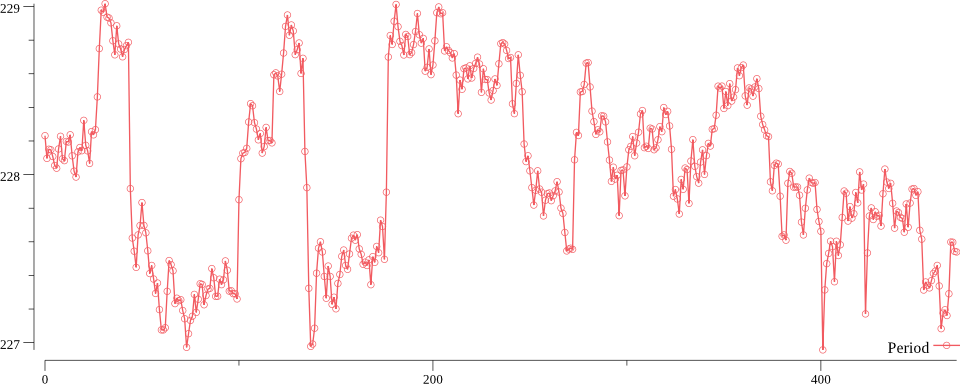
\includegraphics[width=\textwidth]{ErgebnisPeriodeRohdaten}
            \caption{Spannungsverlauf in Volt von "`24.10.2017 15:29:44"' bis "`24.10.2017 15:41:57"'}
            \label{fig:ResultClassificationPeriod}
        \end{figure}

        \begin{figure}[H]
            \centering
            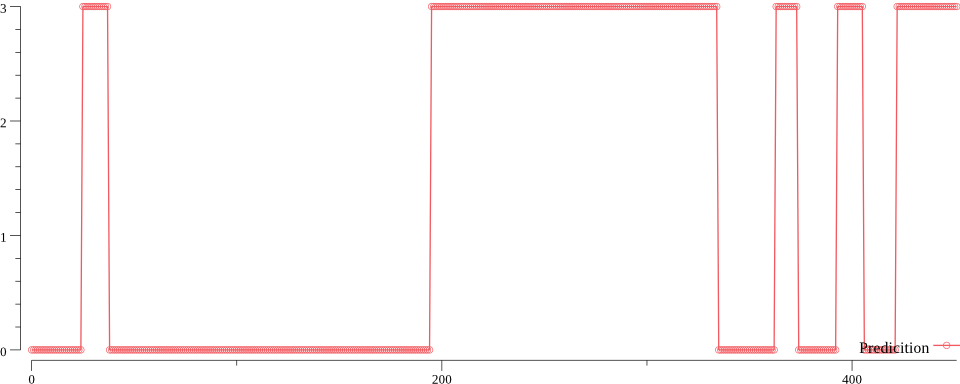
\includegraphics[width=\textwidth]{CNN_ErgebnisKlassifizierung}
            \caption{Klassifizierung mit CNN}
            \label{fig:CNN_RawClassification}
        \end{figure}

        \begin{figure}[H]
            \centering
            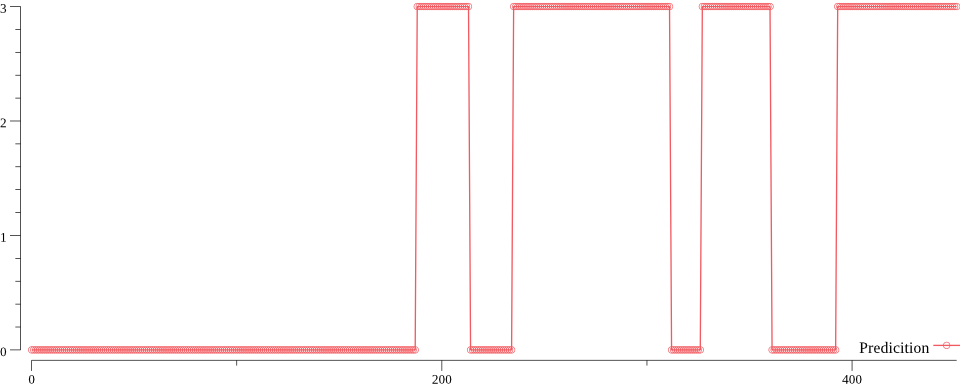
\includegraphics[width=\textwidth]{RNN_ErgebnisKlassifizierung}
            \caption{Klassifizierung mit RNN}
            \label{fig:RNN_RawClassification}
        \end{figure}

        \begin{figure}[H]
            \centering
            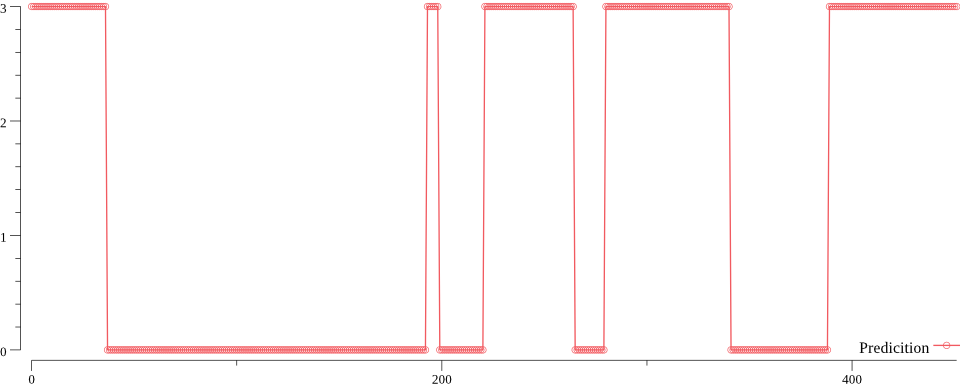
\includegraphics[width=\textwidth]{MIX_ErgebnisKlassifizierung}
            \caption{Klassifizierung mit Mixed RNN und CNN}
            \label{fig:MIX_RawClassification}
        \end{figure}

    \subsection{Ergebnisglättung}
        Eine Möglichkeit die Ungenauigkeit des neuronalen Netzes zu verbessern ist die Auswertung der Ausreißer.
        Durch die Einbeziehung einer weiteren Eigenschaft der Geräte können einige Ausreißer erkannt und beseitigt werden.
        Wie bereits im Abschnitt \ref{Ergebnis} in Paragraph "`Batch"' erwähnt wurde, wird die Größe der Batches klein gehalten damit Geräte mit kleineren Laufzeiten erkannt werden können.
        Diese Laufzeiten können auch für eine weitere Verbesserung verwendet werden.
        Durch die Datenbank(vgl. Kapitel \ref{Messdaten}), welche die manuell klassifizierten Geräte beinhaltet, wird die kürzeste Laufzeit jedes Gerätes ermittelt.
        Diese Laufzeit gibt an wie lange ein Gerät mindestens aktiv war.
        Somit wird diese Eigenschaft eingesetzt um Ausreißer, welche kürzer dauern als die kürzeste Laufzeit, zu beseitigen.
        Daraus ergibt sich für die Abbildung \ref{fig:CNN_RawClassification} eine geglättete Klassifikation, siehe Abbildung \ref{fig:CNN_SmoothClassification}.

        \begin{figure}[H]
            \centering
            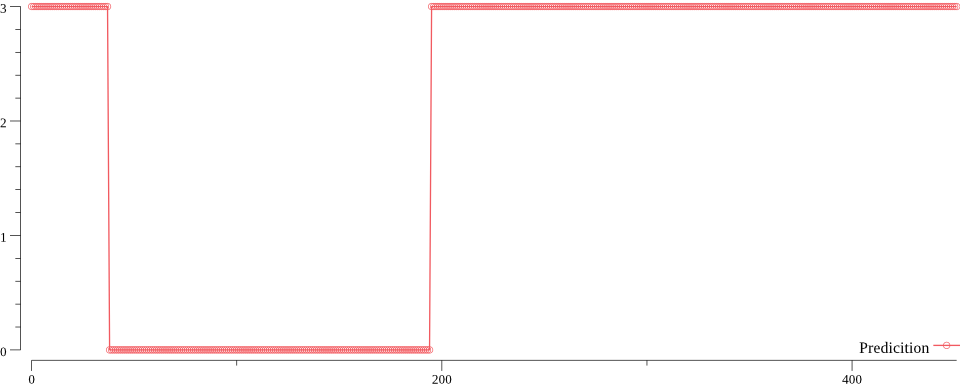
\includegraphics[width=\textwidth]{CNN_ErgebnisKlassifizierung_Smooth}
            \caption{Geglättetes Ergebnis des CNN}
            \label{fig:CNN_SmoothClassification}
        \end{figure}
    
    \subsection{Zusammenfassung}
        Das Ergebnis ist ein neuronales Netz welches mithilfe verschiedener Algorithmen die aktive Laufzeit verschiedener Geräte bestimmen kann.
        Dies bedeutet, dass bestimmt werden kann zu welchen Zeiten welche Geräte aktiv waren und benutzt wurden.
        
        Um weitere Geräte klassifizieren zu können oder die Genauigkeit der bisherigen Geräte zu verbessern, ist es notwendig viel mehr klassifizierte Daten zu erheben.
\chapter{Produktivbetrieb}
    Das aus Kapitel \ref{Ergebnis} resultierende neuronale Netz sowie die Ergebnisauswertung dessen kann bisher nur begrenzt genutzt werden.
    Um diese Funktionen produktiv einsetzten zu können wird eine Schnittstelle zur einfachen Verwendung benötigt.
    
    An diese Schnittstelle werden folgende weitere Vorraussetzungen gestellt:
    \begin{description}
        \item[Echzeitanalyse] Es soll möglich sein Daten, beziehungsweise Batches in Echtzeit zu analysieren.
        \item[Periodenanalyse] Es soll möglich sein für beliebige historische Zeiträume Geräte zu klassifizieren.
        \item[Performance] Es sollte möglich sein lange Zeitreihen mit sehr vielen Daten auch noch in annehmbarer Zeit auszuwerten. Zudem sollte es möglich sein Zeitreihen in Echtzeit zu analysieren.
        \item[Tests] Um Fehler zu verhindern und ein stabiles und sicheres Programm zu entwickeln sollen wichtige fehleranfällige Funktionalitäten getestet werden.
    \end{description}
    
    \subsection{Implementierung}

        \begin{figure}[h]
            \centering
            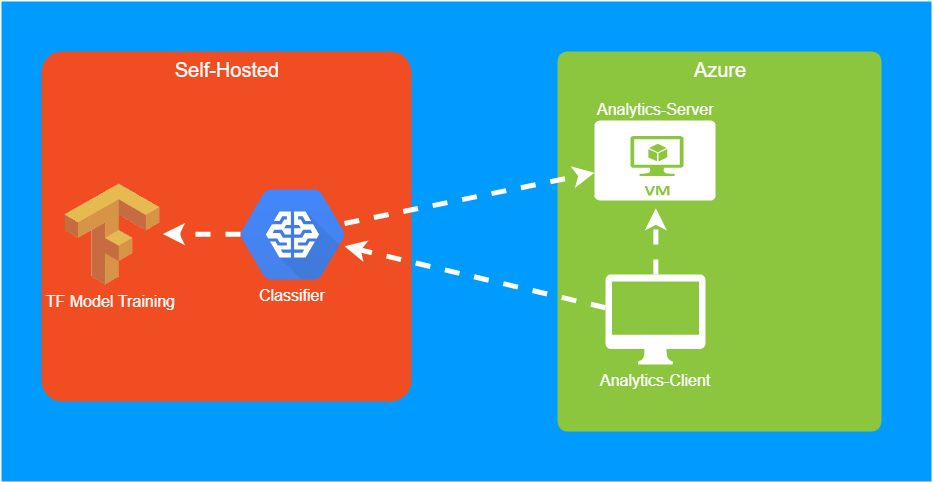
\includegraphics[width=1.0\textwidth]{ArchitectureProduct}
            \caption{Architektur zum Produktivbetrieb \protect\cite{DrawIO}, \protect\cite{Tensorflow}}
            \label{fig:ArchitectureProduct}
        \end{figure}

        Aufgrund besserer Performance und Einheitlichkeit mit der Daten-API (vgl. Analytics-Server in Abbildung \ref{fig:ArchitectureProduct}) wird eine Socekt.IO-API anstatt einer gebräuchlicheren REST-API gewählt.
        Die Spezifikation dieser Schnittstelle wird, wie in Abschnitt \ref{API-Spezifikation} beschrieben, festgelegt. 
        Somit ist die Echtzeitanalyse sowie die Periodenanalyse mit möglichst wenig Mehraufwand abgebildet.
        \newline

        Durch das Verwenden von Tensorflow und dessen Unterstützungseinschränkungen\footnote{https://www.tensorflow.org/install/} steht eine begrenzte Anzhal an Ansätzen zur Wahl.
        Es ist möglich die Architektur auf Python, C oder GoLang aufzubauen.
        Da die Architektur die vorher beschriebenen Anforderungen erfüllen muss und eine einfache Benutzung der neuronalen Netze erlauben sollte, werden mögliche Architekturen auf diese Anforderungen geprüft.
        \newline

        Da der komplette Trainingsprozess bereits in Python implementiert wurde, werden erste Implementierungen dort getestet \footnote{https://github.com/schrodit/wesense-ml/tree/master/prod}.
        Jedoch ist Python schlecht geeignet für viele Anfragen mit großem Rechenaufwand, wie für die Vorbereitung der Daten erforderlich ist.
        Auch konnte das Auslagern der aufwendigen Rechenoperationen keine bessereren Ergebnissen liefern.
        Somit wird entschieden den Produktivbetrieb in GoLang zu implementieren.
        \newline

        Der Einsatz von GoLang kann alle benötigten Anforderungen erfüllen, auch wenn die Einbindung sowie der Support von Tensorflow nicht so gut ausfällt, wie es bei Python der Fall ist.
        Jedoch kann mit GoLang die essentielle Performanceanforderung ohne Probleme erfüllt werden und auch die Stabilität sowie die Fehleranfälligkeit wird dadurch erheblich verbessert.
        Die Implementierung (siehe \footnote{https://github.com/schrodit/wesense-ml/tree/master/go}) besteht aus drei essentiellen Bausteinen, welche in Module (Packages) aufgeteilt sind.
        Diese drei Grundbausteine bestehen aus der Datentransformation, der Klassifikation sowie dem Socket.IO-Server.
        \newline

        Da im Datentransformations-Modul die essentiellen und fehleranfälligen Funktionalitäten implementiert sind, sind Tests für dieses Modul besonders wichtig.
        Hier wird eine Testabdeckung von mehr als 70\% erreicht um die Funktionsfähigkeit sicherzustellen.
        \newline

        Um eine stabile, zuverlässige und fehlerfreie Applikation zu schaffen wird eine \ac{CI}-Umgebung eingeführt.
        Diese \ac{CI}-Umgebung führt bei jedem Commit alle Tests aus, kompiliert das Program und baut einen Docker-Container (siehe \footnote{https://github.com/schrodit/wesense-ml/blob/master/.drone.yml}) in einer isolierten, gleichartigen Umgebung.
        Somit kann eine gleichbleibend gute Qualität der Applikation sichergestellt werden.
    
    \subsection{Deployment}
        Die Bereitstellung der API wird als Docker-Container realisiert.
        Diese Deployment-Strategie bietet viele Vorteile wie Abstraktion von anderen Programmen eines Systems bei wenig Performance-Verlust, welcher bei der Echtzeitanalyse von Nöten ist.
        Außerdem ermöglicht es ein automatisches Deployment mit automatischer Lastverteilung in weitere Docker-Umgebungen.
        Somit wird zur Bereitstellung der API nur eine Docker-Umgebung benötigt und kann sehr einfach auf weitere Server portiert werden.
                

    \subsection{API-Spezifikation}\label{API-Spezifikation}
        \subsubsection{Single Batch}
        \paragraph{Input:}

            \begin{lstlisting}[language=json,firstnumber=1]
Topic: "single-batch"
{
    "data": [
        {
            "u": float,
            "f": float,
            "h3": float,
            "h5": float,
            "h7": float,
            "h9": float,
            "h11": float,
            "h13": float,
            "h15": float,
        },
        .. x Batchsize
    ]
}
            \end{lstlisting}
        
            \paragraph{Output:}
        
            \begin{lstlisting}[language=json,firstnumber=1]
Topic: 'single-prediction'
{
    "data": float //- Prediction of Senseo
}
            \end{lstlisting}
    
        \subsubsection{Period}
            \paragraph{Input:}
    
                \begin{lstlisting}[language=json,firstnumber=1]
Topic: "period"
{
    "data": {
        "start": "DateTime2",
        "end": "DateTime2"
    }
}
                \end{lstlisting}
            
                \paragraph{Output:}
            
                \begin{lstlisting}[language=json,firstnumber=1]
Topic: 'period-prediction'
* Series of Predictions where 0: Senseo, 1: Microwave, 2: Bosch, 3: Undefined, for every second
{
    "data": [
        Int,
        ... end - start
        Int
    ]
}
                \end{lstlisting}

\chapter{Wirtschaftlichkeit}
    Das Ergebnis und die Erkenntnis aus dieser Arbeit kann in verschiedenen Industriebranchen, sowie auch im privaten Gebrauch eingesetzt werden.

    \paragraph{Hersteller von Haushaltsgeräten}
    Falls Hersteller von diversen Haushaltsgeräten auf anonymisierte Strommessdaten aus privaten Haushalten zugreifen können, wäre es möglich Laufzeiten ihrer Geräten zu analysieren.
    Somit kann die Aktivität, beziehungsweise die Benutzung dieser Geräte in Gebieten bestimmt werden. 
    
    Durch präzisere Verbraucherinformationen kann der \ac{CRM}-Prozess eines Unternehmens optimiert werden.
    Durch präzisere Messdaten können Fehlfunktionen klassifiziert werden und so "`Predictive Maintenance"' für die Geräte angeboten werden.

    \paragraph{Privater Gebrauch}
    Für den privaten Gebrauch kann die Aktivität der Geräte dadurch von Vorteil sein, dass intelligent Strom gespart werden kann.
    
    Auch kann eine Art digitaler Marktplatz eingerichtet werden, indem private Kunden Geräte klassifizieren und diese Daten an Unternehmen verkaufen können.

    \paragraph{Energieindustrie}
    In der Energieindustrie können mithilfe dieser Technik einfache Haushaltsgeräte erkannt werden. 
    Mit derselben Technik können auch Störungen sowie spezielle Merkmale eines Stromnetzes erkannt werden. 
    Dadurch kann analysiert werden wann und warum bestimmte Störungen auftreten, wodurch Energiezulieferer besser und schneller auf diese reagieren können.
    \newline

    Wie gezeigt wurde, kann das Ergebnis dieser Arbeit vielfältig in verschiedenen Wirtschaftzweigen eingesetzt werden.
    Um auf dem Markt erfolgreich zu sein, muss jedoch das Ergebnis dieser Arbeit mit mehr Daten trainiert und verbessert werden.
    Da dies jedoch für die Industrieunternehmen kein Problem darstellen sollte, kann diese Arbeit ein Denkanstoß sein.

\listoffigures
\listofalgorithms
\bibliographystyle{plain} 
\bibliography{bib/myBib.bib}
\end{document}